%% 
%% Copyright 2007-2024 Elsevier Ltd
%% 
%% This file is part of the 'Elsarticle Bundle'.
%% ---------------------------------------------
%% 
%% It may be distributed under the conditions of the LaTeX Project Public
%% License, either version 1.3 of this license or (at your option) any
%% later version.  The latest version of this license is in
%%    http://www.latex-project.org/lppl.txt
%% and version 1.3 or later is part of all distributions of LaTeX
%% version 1999/12/01 or later.
%% 
%% The list of all files belonging to the 'Elsarticle Bundle' is
%% given in the file `manifest.txt'.
%% 
%% Template article for Elsevier's document class `elsarticle'
%% with numbered style bibliographic references
%% SP 2008/03/01
%% $Id: elsarticle-template-num.tex 249 2024-04-06 10:51:24Z rishi $
%%
% \documentclass[preprint,12pt]{elsarticle}

%% Use the option review to obtain double line spacing
% \documentclass[authoryear,preprint,review,12pt]{elsarticle}

%% Use the options 1p,twocolumn; 3p; 3p,twocolumn; 5p; or 5p,twocolumn
%% for a journal layout:
%% \documentclass[final,1p,times]{elsarticle}
%% \documentclass[final,1p,times,twocolumn]{elsarticle}
\documentclass[final,3p,times]{elsarticle}
%% \documentclass[final,3p,times,twocolumn]{elsarticle}
%% \documentclass[final,5p,times]{elsarticle}
%% \documentclass[final,5p,times,twocolumn]{elsarticle}

%% For including figures, graphicx.sty has been loaded in
%% elsarticle.cls. If you prefer to use the old commands
%% please give \usepackage{epsfig}

%% The amssymb package provides various useful mathematical symbols
\usepackage{amssymb}
%% The amsmath package provides various useful equation environments.
\usepackage{amsmath}
\usepackage[hidelinks]{hyperref}
\usepackage{algorithmic}
\usepackage{algorithm}
\usepackage{subfigure}
\usepackage{booktabs}
\usepackage{bm}
\input{math_utils}
\usepackage{amssymb}% http://ctan.org/pkg/amssymb
\usepackage{pifont}% http://ctan.org/pkg/pifont
\newcommand{\cmark}{\ding{51}}%
\newcommand{\xmark}{\ding{55}}%
%% The amsthm package provides extended theorem environments
%% \usepackage{amsthm}

%% The lineno packages adds line numbers. Start line numbering with
%% \begin{linenumbers}, end it with \end{linenumbers}. Or switch it on
%% for the whole article with \linenumbers.
%% \usepackage{lineno}

% 自定义颜色和高亮命令

\usepackage{geometry}
\usepackage{booktabs}
\usepackage{multirow}
\usepackage{xcolor}
\usepackage[normalem]{ulem} % normalem 防止改变 \emph 的默认行为
\usepackage{graphicx}
\graphicspath{{../figures_png/}}
\definecolor{myblue}{RGB}{0, 112, 192} % 接近图中的蓝色
\definecolor{revisionblue}{RGB}{0, 90, 180}
\newcommand{\best}[1]{\textbf{\textcolor{red}{#1}}}
\newcommand{\second}[1]{\underline{\textit{\textcolor{myblue}{#1}}}}
\newcommand{\revise}[1]{\textcolor{revisionblue}{#1}}



\journal{Knowledge-Based Systems}

\begin{document}

\begin{frontmatter}

%% Title, authors and addresses

%% use the tnoteref command within \title for footnotes;
%% use the tnotetext command for theassociated footnote;
%% use the fnref command within \author or \affiliation for footnotes;
%% use the fntext command for theassociated footnote;
%% use the corref command within \author for corresponding author footnotes;
%% use the cortext command for theassociated footnote;
%% use the ead command for the email address,
%% and the form \ead[url] for the home page:
%% \title{Title\tnoteref{label1}}
%% \tnotetext[label1]{}
%% \author{Name\corref{cor1}\fnref{label2}}
%% \ead{email address}
%% \ead[url]{home page}
%% \fntext[label2]{}
%% \cortext[cor1]{}
%% \affiliation{organization={},
%%             addressline={},
%%             city={},
%%             postcode={},
%%             state={},
%%             country={}}
%% \fntext[label3]{}

\title{UVHF: Unified Varied-Horizon Time-Series Forecasting with a Multi-Scope Decoder and Balanced Co-Adaptation}

%% use optional labels to link authors explicitly to addresses:
%% \author[label1,label2]{}
%% \affiliation[label1]{organization={},
%%             addressline={},
%%             city={},
%%             postcode={},
%%             state={},
%%             country={}}
%%
%% \affiliation[label2]{organization={},
%%             addressline={},
%%             city={},
%%             postcode={},
%%             state={},
%%             country={}}

\author{Chenhao Ying}
\ead{chenhying01@zju.edu.cn}
\author{Jiangang Lu\corref{cor1}}
\ead{lujg@zju.edu.cn}
%% Author affiliation
\address{{State Key Laboratory of Industrial Control Technology, College of Control Science and Engineering, Zhejiang University},
            {Hangzhou},
            {310027},
            {Zhejiang},
            {China}}



\cortext[cor1]{Corresponding author}

%% Abstract
\begin{abstract}
Most time-series forecasting methods optimize a model for a predefined prediction horizon, whereas practical applications often request forecasts of different lengths from the same history. Under the prevailing horizon-specific paradigm, separate models are optimized for different prediction lengths. This fragments multi-horizon service and can produce inconsistent forecasts for future steps shared across horizon requests. We define unified varied-horizon forecasting as learning one horizon-agnostic trajectory whose nested prefixes serve different request endpoints. This formulation imposes two coupled requirements on decoder design. First, predictions for shared future steps must remain invariant to the requested horizon, a property we term cross-horizon prefix consistency (CHPC). Second, jointly modeling short-, medium- and long-range futures requires the decoder to regulate how broadly history-conditioned information is shared across the future domain. We therefore introduce UVHF, a unified forecasting framework built around a Multi-Scope Decoder (MSD). The MSD constructs region-wise forecasts under multiple sharing scopes and integrates them through target-adaptive allocation into one trajectory, thereby satisfying CHPC by construction. We further develop Balanced Co-Adaptation (BCA), which balances the joint optimization of scope-conditioned forecasts and their allocation through scope-wise supervision and usage regularization. Experiments across seven multivariate benchmarks show that UVHF achieves state-of-the-art accuracy against recent horizon-specific and unified forecasters while serving all supported horizons with a single model. It also offers a favorable trade-off between checkpoint storage and inference memory. Controlled ablations support the proposed components, and generalization studies demonstrate the portability of the MSD across the evaluated backbone families. These results establish output-side multi-scope generation as an effective foundation for unified varied-horizon forecasting.
\end{abstract}

%%Graphical abstract
% \begin{graphicalabstract}
%\includegraphics{grabs}
% \end{graphicalabstract}

%%Research highlights
\begingroup
\makeatletter
\def\@title{\small UVHF: Unified Varied-Horizon Time-Series Forecasting with a Multi-Scope Decoder and Balanced Co-Adaptation}
\makeatother
\begin{highlights}
\item Unified varied-horizon forecasting is formalized through nested trajectory prefixes.
\item A Multi-Scope Decoder adaptively combines forecasts from multiple sharing scopes.
\item Balanced Co-Adaptation jointly optimizes scope forecasts and their allocation.
\item One model achieves state-of-the-art accuracy across seven forecasting benchmarks.
\end{highlights}
\endgroup

%% Keywords
\begin{keyword}
Time series forecasting,
Unified varied-horizon forecasting,
Cross-horizon prefix consistency,
Multi-Scope Decoder,
Balanced Co-Adaptation,
Adaptive forecast generation.
\end{keyword}

\end{frontmatter}

%% Add \usepackage{lineno} before \begin{document} and uncomment
%% following line to enable line numbers
%% \linenumbers

%% main text

%% Use \section commands to start a section

%% BEGIN INLINED UVHF MAIN TEXT
\section{Introduction}
\label{sec:introduction}


Multi-horizon forecasts support decisions over multiple planning ranges, from short-term control to long-term scheduling \citep{zeng2023dlinear}. Yet most long-term time-series forecasting models and benchmark protocols remain horizon-specific: a separate model is trained for each forecast horizon $H$, such as 96, 192, 336, and 720 steps \citep{nie2023patchtst,liu2024itransformer}. Recent work, including ElasTST\citep{zhang2024elastst} and time-series foundation models such as TimesFM\citep{das2024timesfm} and Time-MoE\citep{shi2025timemoe}, has begun to support varied or flexible forecasting horizons through autoregressive and universal-generation designs \citep{liu2024timer,ansari2024chronos,woo2024moirai}. However, these efforts remain sparse relative to the extensive horizon-specific literature and have not yet established varied-horizon forecasting as an explicit task with systematic problem analysis and targeted decoder design. In this work, we investigate how the decoder should organize output-side representations across different parts of the future domain.

The horizon-specific protocol fragments forecasting into independent predictors. As illustrated in Fig.~\ref{fig:conceptual-problems}a, models trained for different horizons can assign different values to the same future time step, despite identical history and forecast origin. Their outputs can therefore disagree on overlapping future targets rather than form nested views of a common trajectory. Supporting several horizons further entails separate training, checkpoint storage, deployment and maintenance.

To formalize a unified alternative, we define \textbf{unified varied-horizon forecasting} as the setting in which one model serves different request endpoints through a shared prediction trajectory. The task learns a single horizon-agnostic mapping from observed history and future-step index to prediction. Under this mapping, a future-step prediction depends on the history and its step index, but not on the requested horizon. For any $H_1<H_2$, predictions over steps $1{:}H_1$ therefore remain identical under both requests. We call this requirement \textbf{cross-horizon prefix consistency (CHPC)}.

CHPC specifies how forecasts at different horizons should relate, but not how a decoder should generate different future regions. Most architectural advances focus on history encoding, while the output stage often uses a uniform mechanism for all future steps \citep{zhou2021informer,wu2021autoformer,zhou2022fedformer,liu2022nonstationary}. Such a decoder fixes the sharing extent, that is, how broadly a history-conditioned latent state is reused before step-specific generation. Broad sharing can capture persistent trajectory structure but may smooth local variations. Finer sharing offers greater step-specific flexibility but weaker structural regularization. The preferred balance can vary across samples, variables and future regions, making a fixed extent inadequate for the full forecast domain. Fig.~\ref{fig:conceptual-problems}b summarizes this output-side heterogeneity, which we term \textbf{future-region sharing-demand heterogeneity}. We examine this problem in greater detail in Section~\ref{sec:problem-formulation}.



\begin{figure*}[t]
\centering
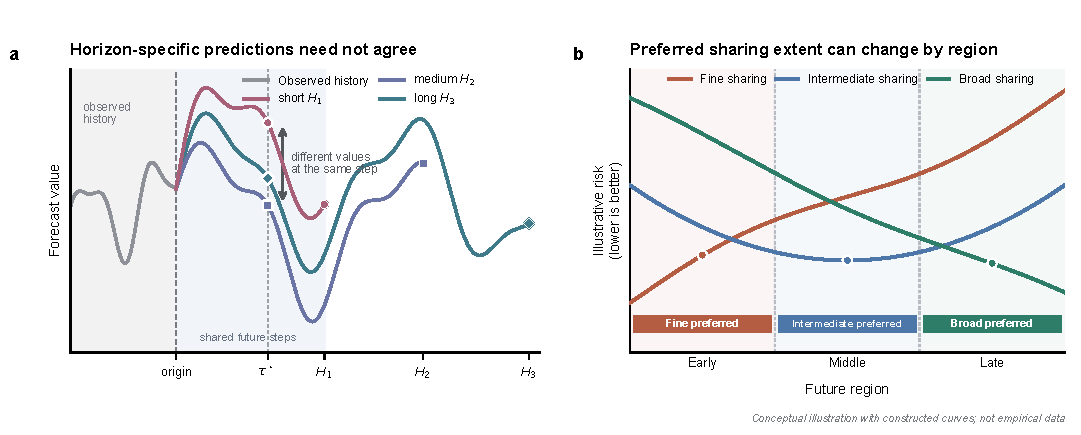
\includegraphics[width=1.00\textwidth]{figure_01_conceptual_problem.pdf}
\caption{Two challenges in unified varied-horizon forecasting. \textbf{a}, Horizon-specific predictors may disagree at the same future time step $\tau^\star$ despite identical observed history. \textbf{b}, The sharing extent associated with the lowest risk can vary across future regions.}
\label{fig:conceptual-problems}
\end{figure*}


Motivated by this heterogeneity, we introduce \textbf{UVHF}, a unified forecasting framework comprising a \textbf{Multi-Scope Decoder (MSD)} and \textbf{Balanced Co-Adaptation (BCA)}. The MSD assigns each scope a dedicated history projection within one scope-indexed forecast field. Each scope specifies the number of future steps over which a history-conditioned latent state is reused. Target-adaptive allocation then integrates the scope-conditioned forecasts for each sample, variable and future step. The resulting trajectory can adapt its sharing composition across future regions while retaining a single horizon-agnostic prediction function. BCA supports joint learning by supplying direct prediction signals to every scope and regulating aggregate scope usage during optimization. It operates only during training, adds no inference parameters or paths, and preserves the CHPC-compliant forward computation of UVHF.

The contributions of our work are summarized as follows:

\begin{enumerate}
\item We formulate unified varied-horizon forecasting as a forecasting system in which CHPC is a basic requirement, and identify future-region sharing-demand heterogeneity as an output-side challenge.
\item We introduce UVHF and its Multi-Scope Decoder, which integrates forecasts generated under multiple sharing scopes through target-adaptive allocation.
\item We develop Balanced Co-Adaptation to support balanced scope learning without increasing inference-time complexity.
\end{enumerate}

Experiments across datasets from multiple application domains show that UVHF achieves state-of-the-art performance among the evaluated baselines and outperforms separately trained horizon-specific forecasters. Component-wise ablations support the utility of the proposed components, and generalization studies demonstrate the portability of the MSD across the evaluated backbone families.

\section{Related Work}
\label{sec:related-work}


\subsection{Fixed-horizon multi-step forecasting}


Multi-step forecasting has traditionally assumed a fixed forecast horizon and differs in how predictions within that horizon are generated. Recursive forecasting iterates one one-step model and feeds predictions back as inputs, which can accumulate errors \citep{taieb2014boosting}. Direct forecasting instead trains a separate model for each future step, avoiding recursive propagation but increasing estimation variance and weakening dependencies among future outputs \citep{taieb2014boosting}. The multiple-input multiple-output (MIMO) strategy predicts the complete future vector with one multi-output model. The direct--MIMO (DIRMO) strategy instead partitions the horizon into blocks and assigns one multi-output model to each block \citep{bontempi2008mimo,taieb2012review,green2025stratify}. These strategies primarily trade error propagation, estimation variance, output dependence and computational cost within a prespecified horizon.

Modern long-term forecasting benchmarks largely use fixed-window, MIMO-like prediction. DLinear, PatchTST and iTransformer map a history representation to one configured prediction length; standard evaluations train separate models for horizons 96, 192, 336 and 720 \citep{zeng2023dlinear,nie2023patchtst,liu2024itransformer}. This protocol optimizes each horizon independently but does not require agreement on overlapping future targets. Unified varied-horizon forecasting instead uses one model to serve multiple request endpoints and returns prefix-consistent views of one predicted trajectory.

\subsection{Unified varied-horizon forecasting}


Advances in time-series foundation models have encouraged models that operate across forecasting tasks or output lengths. TimesFM uses decoder-only pretraining across datasets, granularities and horizons, while Timer and Time-MoE generate flexible forecast lengths autoregressively \citep{das2024timesfm,liu2024timer,shi2025timemoe}. Chronos and Moirai further extend pretrained forecasting through tokenized probabilistic generation and universal masked-encoder training, respectively \citep{ansari2024chronos,woo2024moirai}. UniTS accommodates heterogeneous time-series tasks through task tokenization \citep{gao2024units}. Although these models support multiple horizons or task specifications, they primarily pursue universal pretraining, task unification or scalable generation without systematically treating unified varied-horizon forecasting as a distinct task. ElasTST is a notable exception. It combines structured attention masks, tunable RoPE, multi-scale history patches and horizon reweighting to improve robustness across inference horizons \citep{zhang2024elastst}. Its multi-scale mechanism, however, varies history-patch resolution rather than the output-side extent of state sharing. Our work targets this complementary problem by formalizing CHPC and modeling how state-sharing demand changes across future regions.

\subsection{Forecast generation and output-side modeling}


Most recent forecasting architectures concentrate on extracting and representing information from the observed history, for example through decomposition, frequency enhancement, cross-dimension attention or convolutional token modeling \citep{wu2021autoformer,zhou2022fedformer,liu2022nonstationary,zhang2023crossformer,luo2024moderntcn}. Their output stages often remain shallow fixed-window projections. DLinear directly maps temporal inputs to future steps, while PatchTST and iTransformer project patch-level or variate-level representations through linear prediction heads \citep{zeng2023dlinear,nie2023patchtst,liu2024itransformer}. Consequently, the forecasting phase is commonly treated as a readout of an increasingly sophisticated history Encoder rather than a separate modeling problem.

Beyond shallow output projections, several studies have introduced structured mechanisms for forecast generation. TFFS combines common and step-specific future features, N-BEATS and N-HiTS synthesize forecasts through basis expansion or hierarchical interpolation, and Implicit Forecaster composes predicted waves into a global trajectory \citep{zhang2024tffs,oreshkin2020nbeats,challu2023nhits,li2025implicit}. These methods establish forecast generation as a first-class design problem rather than a passive readout. However, their cross-step sharing structure is predefined by the decoder topology. The MSD in UVHF instead makes state-sharing extent explicit and constructs region-local forecasts under multiple scopes before step-specific generation.

\subsection{Multi-scale forecasting and adaptive allocation}


Most multi-scale forecasters extract and combine temporal dependencies from the observed history to form hierarchical representations. SCINet recursively interacts with downsampled subsequences, while N-HiTS couples multi-rate sampling with hierarchical synthesis \citep{liu2022scinet,challu2023nhits}. Pathformer selects pathways over input patch scales, whereas TimeMixer mixes decomposed histories with scale-specific predictors \citep{chen2024pathformer,wang2024timemixer}. These methods define scale through input resolution, frequency structure or complete prediction branches. The MSD adopts an output-side perspective. Starting from one History State, it generates forecasts under multiple state-sharing scopes and allocates these granularities according to each future target.

Expert-based forecasters also use conditional allocation, but route among components with different modeling functions. MoLE mixes complete linear-centric forecasters, whereas FreqMoE assigns frequency components to experts \citep{ni2024mole,liu2025freqmoe}. Time-MoE and Moirai-MoE instead activate sparse internal experts within foundation models \citep{shi2025timemoe,liu2025moiraimoe}. The scopes in the MSD are jointly learned forecast-generation paths with shared Encoder and Region-to-Step Forecast Generator parameters. Scope Projections construct information pools tied to explicit state-reuse extents, and Scope Probabilities allocate these sharing granularities for each target. BCA jointly optimizes the resulting scope-indexed forecast field and its allocation process. This output-side interpretation underlies the sharing-demand heterogeneity formalized in Section 3.

\section{Problem Formulation and Empirical Motivation}
\label{sec:problem-formulation}


The preceding discussion shows that unified varied-horizon forecasting involves more than sharing parameters across prediction lengths. A unified forecaster should return coherent predictions for future steps shared by different horizon requests, while its decoder must determine how predictive information is shared across the future domain. We now formalize these two issues and examine them through controlled empirical analyses, which motivate the decoder design developed in Section 4.

\subsection{Unified varied-horizon forecasting and cross-horizon prefix consistency}


Consider two forecasting requests with horizons $H_i<H_j$ issued from the same observed history. Their first $H_i$ steps refer to identical future targets and should therefore receive identical predictions. We formalize this requirement below.

At forecast origin $o$, let

\begin{equation}
\mathbf X_o
=
\left[\mathbf x_{o-L+1},\ldots,\mathbf x_o\right]
\in\mathbb R^{L\times C},
\qquad
\mathbf Y_o^{(H)}
=
\left[y_{o+\tau,c}\right]_{\tau=1,\ldots,H;\ c=1,\ldots,C}
\in\mathbb R^{H\times C}.
\end{equation}


Here, $\mathbf X_o$ is a length-$L$ multivariate history, and $\mathbf Y_o^{(H)}$ contains the next $H$ targets for $C$ variables. Let $\mathcal H=\{H_1,\ldots,H_M\}$ denote the supported horizons and $T=\max\mathcal H$. The horizon $H$ specifies the request endpoint, whereas $\tau$ indexes a particular future step. Thus, target $(\tau,c)$ is shared by all requests with $H\geq\tau$.

This shared-target relation defines \textbf{cross-horizon prefix consistency (CHPC)}. Let $\widehat y_{o+\tau,c}^{(H)}$ denote the prediction returned for target $(\tau,c)$ under a request with horizon $H$. Given identical history, forecast origin and preprocessing, CHPC requires

\begin{equation}
\widehat y_{o+\tau,c}^{(H_i)}
=
\widehat y_{o+\tau,c}^{(H_j)},
\qquad
\forall\,H_i,H_j\in\mathcal H,\ H_i<H_j,\quad
1\leq\tau\leq H_i,\quad
1\leq c\leq C.
\end{equation}


Conventional long-term forecasting learns an independent predictor $f_{\theta_H}$ for each horizon. Because both parameters and optimization are horizon-specific, these predictors are not constrained to satisfy CHPC on their overlapping outputs.

A varied-horizon forecaster should instead use a single \textbf{future-step-indexed prediction function} $g_\theta(\mathbf X_o,\tau,c)$ and construct an $H$-step forecast as

\begin{equation}
\widehat{\mathbf Y}_o^{(H)}
=
\left[
g_\theta(\mathbf X_o,\tau,c)
\right]_{\tau=1,\ldots,H;\ c=1,\ldots,C}.
\end{equation}


For a varied-horizon forecaster, all horizon requests query the same function at a shared target, so CHPC holds by construction. Changing the requested horizon alters only the returned prefix length, and each request becomes a nested view of one predicted trajectory.

\subsection{Horizon-specific prefix inconsistency}


Independently trained horizon-specific predictors may agree on some overlapping outputs, but their objectives do not enforce CHPC. We refer to a violation of CHPC as \textbf{cross-horizon prefix inconsistency} and quantify its magnitude through prediction disagreement on aligned histories and shared future targets.

At origin $o$, let $\widehat{\mathbf Y}_{o}^{(H_i)}\in\mathbb R^{H_i\times C}$ and $\widehat{\mathbf Y}_{o}^{(H_j)}\in\mathbb R^{H_j\times C}$ denote forecasts from independently trained models, where $H_i<H_j$. We define their \textbf{cross-horizon prefix disagreement (CHPD)} as

\begin{equation}
\operatorname{CHPD}_o(H_i,H_j)
=
\frac{1}{H_iC}
\sum_{\tau=1}^{H_i}
\sum_{c=1}^{C}
\left|
\widehat y_{o+\tau,c}^{(H_i)}
-
\widehat y_{o+\tau,c}^{(H_j)}
\right|.
\end{equation}


CHPD measures the mean absolute difference over the shared prefix in the original data scale. To aggregate variables with different magnitudes, we further define normalized CHPD (NCHPD):

\begin{equation}
\operatorname{NCHPD}(H_i,H_j)
=
\frac{1}{|\mathcal O|C}
\sum_{o\in\mathcal O}
\sum_{c=1}^{C}
\frac{
\frac{1}{H_i}\sum_{\tau=1}^{H_i}
\left|
\widehat y_{o+\tau,c}^{(H_i)}
-
\widehat y_{o+\tau,c}^{(H_j)}
\right|
}{
\sigma_c^{\mathrm{train}}+\epsilon
}.
\end{equation}


Here, $\mathcal O$ denotes the aligned evaluation origins, $\sigma_c^{\mathrm{train}}$ is the train-split standard deviation of variable $c$, and $\epsilon$ is the fixed numerical stabilizer used in the computation. All comparisons use identical histories, forecast origins, scalers and overlapping target indices.

To visualize this inconsistency, we compare multi-horizon forecasts from DLinear models independently optimized on ETTh2 \citep{zeng2023dlinear}. Fig.~\ref{fig:prefix-disagreement}a shows that their predictions diverge over the same 96 future steps: relative to the $H=720$ forecast, the forecasts for $H\in\{96,192,336\}$ differ by 2.51, 2.16 and 2.40 in mean absolute raw scale, respectively.

We further evaluate all 2,161 aligned ETTh2 validation origins and variables, with the resulting NCHPD matrix shown in Fig.~\ref{fig:prefix-disagreement}b. NCHPD is non-zero for every horizon pair and is more pronounced between the longest and shorter requested horizons: the $H=96$, $H=192$ and $H=336$ comparisons with $H=720$ yield 0.0406, 0.0365 and 0.0366, whereas pairs among the three shorter horizons range from 0.0148 to 0.0166. These results show that the independently optimized DLinear models evaluated here fail to form a prefix-consistent prediction trajectory, reflecting a structural limitation of horizon-specific forecasting: independently optimized models are not constrained to agree on shared future targets.



\begin{figure*}[t]
\centering
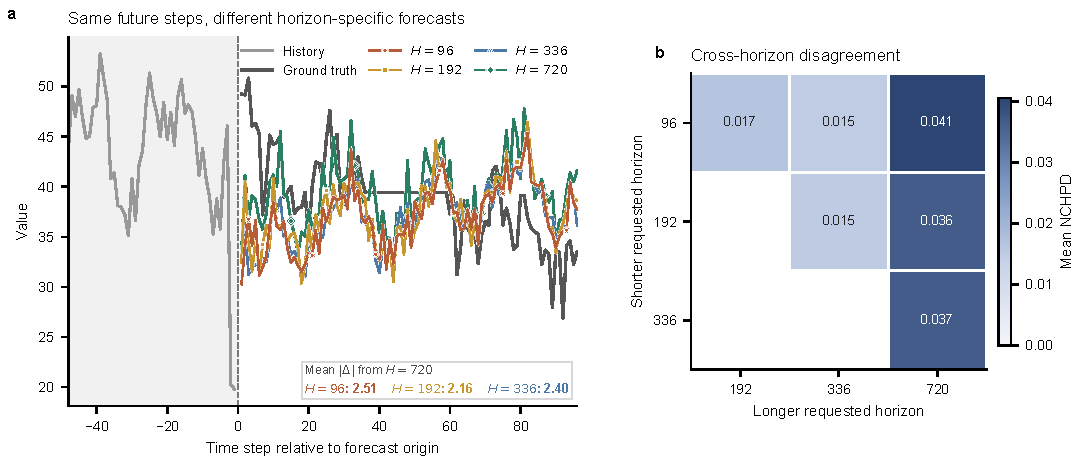
\includegraphics[width=0.96\textwidth]{figure_02_prefix_disagreement.pdf}
\caption{Horizon-specific forecasts disagree on shared future steps. \textbf{a}, Selected ETTh2 validation trajectory from independently trained DLinear models for horizons 96, 192, 336 and 720; the inset reports differences from the $H=720$ forecast. \textbf{b}, NCHPD over 2,161 aligned ETTh2 validation origins and all variables.}
\label{fig:prefix-disagreement}
\end{figure*}


\subsection{Future-region sharing-demand heterogeneity}


CHPC specifies how predictions from different horizon requests should relate, but it does not determine how a unified decoder should construct the shared future trajectory. Simply adapting an architecture designed for one fixed horizon leaves this output-side requirement unresolved: a varied-horizon forecaster must learn from requests spanning short to long endpoints while producing one prefix-consistent trajectory. The decoder is therefore central to how predictive information is organized across the future domain, particularly in determining how broadly each history-conditioned state is reused before step-specific prediction.

We use the \textbf{sharing extent} $s$ to denote the number of future steps that reuse one latent state. A \textbf{future region} $\mathcal B_b\subseteq\{1,\ldots,T\}$ is a contiguous subset of the maximum future domain rather than a requested horizon. Broad sharing can capture persistent trajectory structure but may smooth local variations, whereas fine sharing offers greater local flexibility with weaker cross-step regularization. We refer to variation in the preferred extent across regions as \textbf{future-region sharing-demand heterogeneity}.

To isolate this factor, we construct capacity-matched single-extent predictors that differ only in sharing extent; all other architecture, training and evaluation settings remain identical.

For aligned origin $o$, we define the \textbf{future-region prediction risk} of sharing extent $s$ over region $\mathcal B_b$ as the empirical squared-error loss

\begin{equation}
R_{o,b,s}
=
\frac{1}{|\mathcal B_b|C}
\sum_{\tau\in\mathcal B_b}
\sum_{c=1}^{C}
\left(
\widehat y_{o+\tau,c}^{(s)}
-
y_{o+\tau,c}
\right)^2.
\end{equation}


For a given origin and region, $R_{o,b,s}$ averages squared errors over the region's future steps and variables. Lower $R_{o,b,s}$ indicates that extent $s$ better matches region $\mathcal B_b$ within the controlled family; a region-dependent preference appears when $s_{o,b}^{\star}=\arg\min_sR_{o,b,s}$ changes with $b$.

We evaluate the five predictors with $s\in\{1,8,32,128,720\}$ across 12 contiguous 60-step future regions on ETTm2. Fig.~\ref{fig:sharing-heterogeneity}a reports the percentage excess prediction risk of each extent above the lowest-risk extent within each region, with outlined squares marking the region-wise winners. The preferred extents vary across the future domain: each of the five extents wins two or three regions, and the mean best-versus-second-best margin reaches 10.266\%. No fixed extent minimizes prediction risk throughout this controlled example, supporting heterogeneous sharing demand across future regions.



\begin{figure*}[t]
\centering
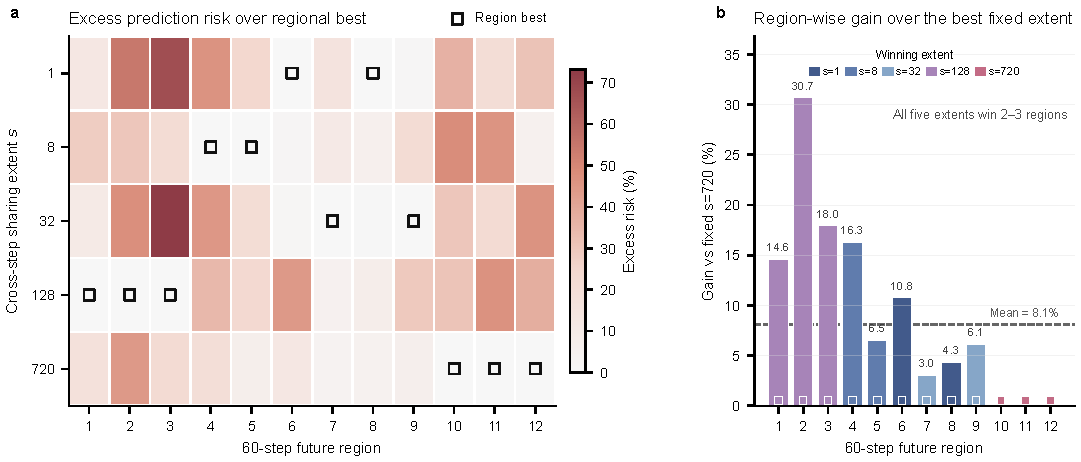
\includegraphics[width=0.96\textwidth]{figure_03_sharing_heterogeneity.pdf}
\caption{Sharing preferences vary across future regions. \textbf{a}, Percentage excess prediction risk of five capacity-matched single-extent predictors on a selected ETTm2 validation example; squares mark regional winners. \textbf{b}, MSE reduction from regional selection relative to the fixed extent $s=720$; dashed line, mean over 12 regions.}
\label{fig:sharing-heterogeneity}
\end{figure*}


Fig.~\ref{fig:sharing-heterogeneity}b quantifies the performance upper bound associated with these region-wise preferences. Relative to the best fixed extent ($s=720$), selecting the lowest-risk extent separately for each region reduces average MSE by 8.112\%. Because the regional winners are selected using validation labels across separately trained predictors, this value represents descriptive oracle headroom rather than the realized gain of a learned decoder. Within this controlled example, its magnitude nevertheless shows that one fixed extent can leave meaningful region-specific headroom, motivating a decoder that can adapt sharing across the future domain.

\section{UVHF Framework}
\label{sec:method}


Section 3 established two decoder-side requirements for unified varied-horizon forecasting. Predictions for a shared future target should be invariant to the requested horizon, while the decoder should not impose one latent-state sharing extent on the entire future domain. UVHF addresses these requirements through two coordinated components. Its \textbf{Multi-Scope Decoder (MSD)} constructs one future-step-indexed trajectory from multiple sharing granularities, and \textbf{Balanced Co-Adaptation (BCA)} jointly optimizes the scope-indexed forecast field and its allocation process.

\subsection{Architecture overview}


Fig.~\ref{fig:uvhf-method} summarizes the forward computation of the MSD, which comprises a \textbf{Scope Forecasting Path} and a \textbf{Target-Adaptive Allocation Path}. The decoder consumes a variable-wise History State rather than relying on a particular Encoder. Any Encoder that models temporal patch tokens and returns the required tensor interface can therefore serve as its backbone. This interface covers the patch-based Encoder family commonly used in time-series forecasting \citep{nie2023patchtst,zhang2023crossformer}. Given a History Series $\mathbf X\in\mathbb R^{B\times L\times C}$, Patchify and the Encoder produce $\mathbf R\in\mathbb R^{B\times C\times R}$. The Scope Forecasting Path constructs region-wise predictions under each sharing scope and assembles them into $\mathcal F_\theta(\mathbf X)\in\mathbb R^{B\times C\times T\times S}$. The Target-Adaptive Allocation Path then determines how each future target draws on these sharing granularities.

The Target-Adaptive Allocation Path combines a projected History State with the Future Coordinate $\boldsymbol\phi_\tau$ and produces Scope Probabilities $\boldsymbol\Pi\in\mathbb R^{B\times C\times T\times S}$. Weighted contraction with the scope-indexed forecast field yields one trajectory $\widehat{\mathbf Y}\in\mathbb R^{B\times T\times C}$. For an $H$-step request, the MSD evaluates only the region--target pairs intersecting the first $H$ future steps. Shared targets retain the same region-local computation across request endpoints, so varying $H$ changes the evaluated extent while preserving all overlapping predictions. UVHF thereby supports variable-length outputs and satisfies CHPC by construction.

The Scope-conditioned Forecasts and Scope Probabilities are optimized jointly. BCA separates two training roles: the Uniform-Prefix Forecasting Loss optimizes varied-horizon prediction, while the Scope-Wise Forecasting Loss and Allocation-Balance Regularizer stabilize multi-scope learning.



\begin{figure*}[t]
\centering
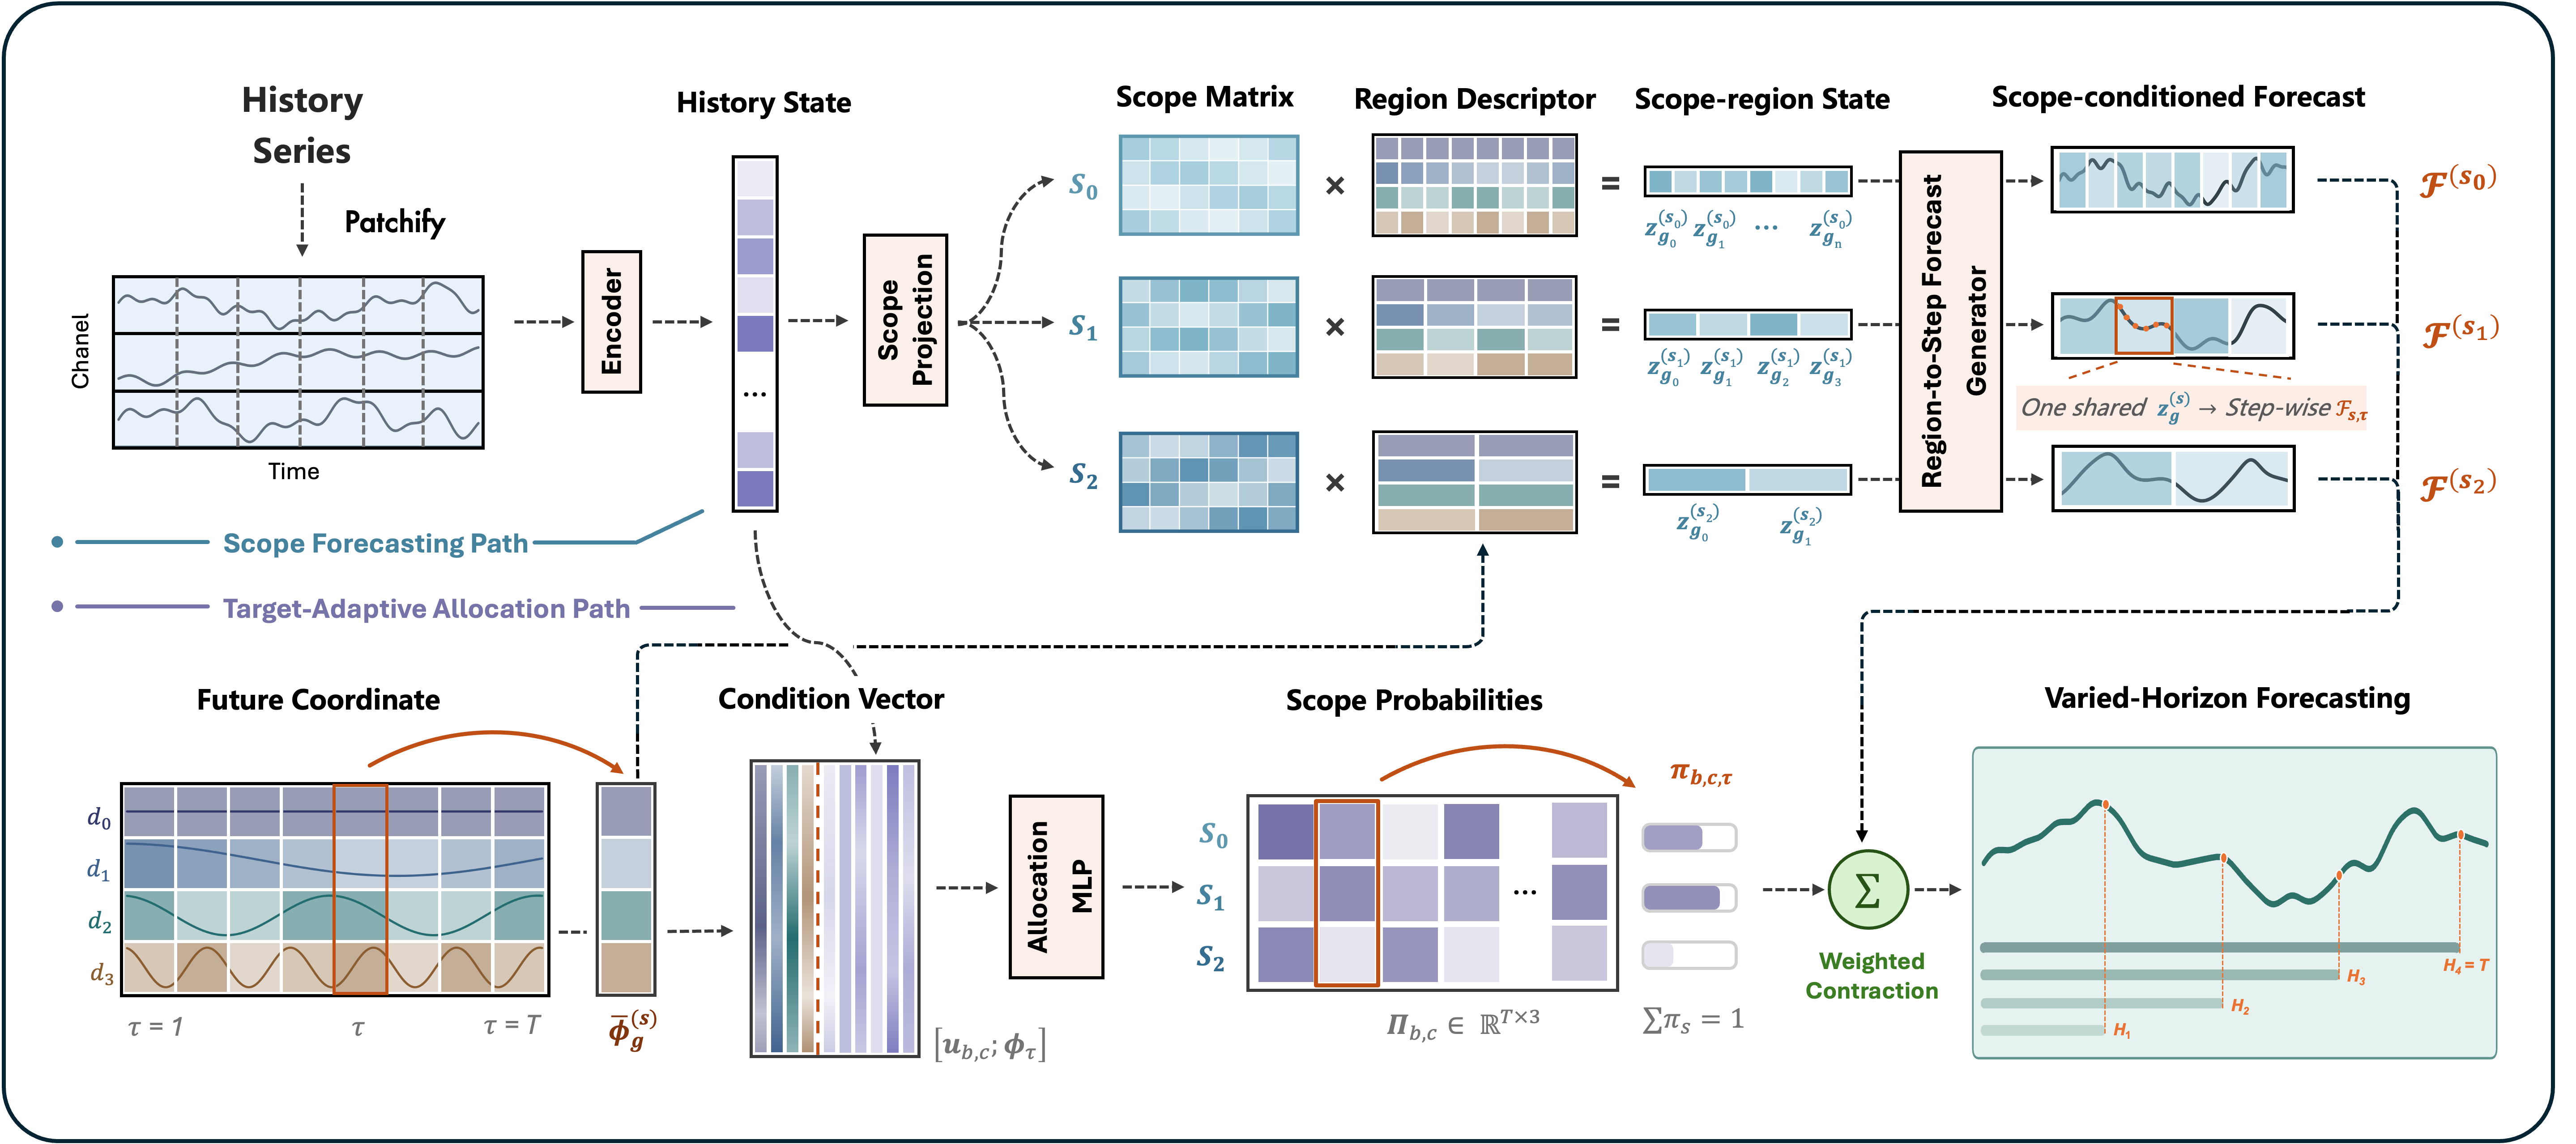
\includegraphics[width=1.00\textwidth]{figure_04_uvhf_msd_overview.png}
\caption{The Multi-Scope Decoder in UVHF. Scope-conditioned forecasts are generated region-wise and integrated through target-adaptive allocation into a prefix-consistent trajectory.}
\label{fig:uvhf-method}
\end{figure*}


\subsection{History state and future coordinate}


The MSD begins with the History State and Future Coordinate shown on the left of Fig.~\ref{fig:uvhf-method}. The History Series is normalized per variable, divided into $P$ patches by Patchify and processed by the shared Encoder. This produces $\mathbf Z\in\mathbb R^{B\times C\times P\times D_e}$, which is flattened over its patch and embedding dimensions:

\begin{equation}
\mathbf Z
=
\mathcal E\!\left(\mathcal N(\mathbf X)\right),
\qquad
\mathbf r_{b,c}
=
\operatorname{vec}(\mathbf Z_{b,c})
\in\mathbb R^R,
\qquad
R=PD_e.
\end{equation}


Collecting $\mathbf r_{b,c}$ over samples and variables gives the History State $\mathbf R=[\mathbf r_{b,c}]\in\mathbb R^{B\times C\times R}$. The preserved variable axis provides one history representation for each sample-variable pair, which is used by both decoder paths.

The History State summarizes the observed series, but a unified decoder must also identify where each prediction lies in the future domain. Using the requested horizon for this purpose would assign different conditioning contexts to the same target under different requests. The MSD therefore introduces a \textbf{Future Coordinate} for every future step. This fixed coordinate supplies a horizon-independent target identity and a common positional basis for regions at different scopes. It also allows the Target-Adaptive Allocation Path to vary its scope preference across future steps.

Formally, the Future Coordinate is the field $\boldsymbol\Phi=[\boldsymbol\phi_1,\ldots,\boldsymbol\phi_T]^\top\in\mathbb R^{T\times D_q}$. We construct it from low-order discrete cosine functions, which provide smooth coordinate channels at progressively finer temporal frequencies. For $d=0,\ldots,D_q-1$, we first define

\begin{equation}
\widetilde\phi_{\tau,d}
=
\cos\!\left(
\frac{\pi(\tau-\tfrac12)d}{T}
\right).
\end{equation}


The constant coordinate is $\phi_{\tau,0}=1$. Each nonconstant coordinate is centered over the future domain and scaled as

\begin{equation}
\phi_{\tau,d}
=
\sqrt{2}
\left(
\widetilde\phi_{\tau,d}
-
\frac{1}{T}
\sum_{j=1}^{T}
\widetilde\phi_{j,d}
\right),
\qquad d\geq 1.
\end{equation}


The constant channel preserves a global reference, while the centered nonconstant channels distinguish positions across the future domain. The Future Coordinate field serves two roles. Region-wise averaging produces the Region Descriptors used to generate Scope-conditioned Forecasts, whereas the unpooled coordinate $\boldsymbol\phi_\tau$ identifies the individual target in the Condition Vector used for Scope Probabilities.

\subsection{Generation of scope-conditioned forecasts}


The Scope Forecasting Path contains $S$ parallel scope lines, one for each sharing scope in $\mathcal S=\{s_1,\ldots,s_S\}$. Each scope has its own parameterized Scope Projection, which maps the History State into a dedicated Scope Matrix:

\begin{equation}
\mathbf M_{b,c}^{(s)}
=
\operatorname{reshape}_{D_q\times K}
\left(
\mathbf r_{b,c}\mathbf W^{(s)}
+
\mathbf b^{(s)}
\right)
\in\mathbb R^{D_q\times K}.
\end{equation}


The matrix form preserves a Future-Coordinate axis and a latent-mode axis, allowing Region Descriptors to query scope-specific history information at different future locations without assigning a separate prediction head to every region.

For a scope $s$, the future domain is divided into contiguous regions

\begin{equation}
\mathcal G_g^{(s)}
=
\{(g-1)s+1,\ldots,gs\},
\qquad
g=1,\ldots,T/s.
\end{equation}


The Future Coordinate within each region is averaged to form the Region Descriptor, which provides a compact positional summary for region-wise state construction:

\begin{equation}
\overline{\boldsymbol\phi}_g^{(s)}
=
\frac{1}{s}
\sum_{\tau\in\mathcal G_g^{(s)}}
\boldsymbol\phi_\tau
\in\mathbb R^{D_q}.
\end{equation}


The Region Descriptor selects and combines information from this matrix through a coordinate contraction, producing the region-wise Scope-region State

\begin{equation}
\mathbf z_{b,c,g}^{(s)}
=
\left(\overline{\boldsymbol\phi}_g^{(s)}\right)^\top
\mathbf M_{b,c}^{(s)}
\in\mathbb R^K.
\end{equation}


Once the Scope Matrix is available, each Scope-region State depends only on the descriptor of its own region. Regions can therefore be evaluated separately and in parallel, although they draw on the same scope-specific history information. All future steps in $\mathcal G_g^{(s)}$ reuse $\mathbf z_{b,c,g}^{(s)}$. A finer scope constructs more region states and limits reuse to shorter intervals, whereas a broader scope shares each state over a longer interval. Scope therefore defines the cross-step reuse pattern.

The Region-to-Step Forecast Generator converts each shared Scope-region State into step-wise predictions. Let $g_s(\tau)$ denote the region containing step $\tau$. The generator is shared across scopes and regions, and uses step-specific vectors $\mathbf a_\tau,\mathbf n_\tau\in\mathbb R^K$ and bias $\beta_\tau$ to define

\begin{equation}
\mathcal F_{b,c,\tau,s}
=
\left\langle
\mathbf a_\tau,
\mathbf z_{b,c,g_s(\tau)}^{(s)}
\right\rangle
+
\left\langle
\mathbf n_\tau,
\operatorname{GELU}\!\left(
\mathbf z_{b,c,g_s(\tau)}^{(s)}
\right)
\right\rangle
+
\beta_\tau.
\end{equation}


Concatenating the separately generated regions gives the Scope-conditioned Forecast $\mathcal F^{(s)}$ for scope $s$. Collecting these forecasts produces the scope-indexed field $\mathcal F_\theta(\mathbf X)\in\mathbb R^{B\times C\times T\times S}$. The MSD constructs this field as a unified decoder through scope-specific projections and a shared Encoder and Region-to-Step Forecast Generator. Parameter sharing couples forecast generation across scopes while avoiding duplicated Encoder computation and generator parameters.

\subsection{Target-adaptive scope allocation}


Different future targets may require information organized at different sharing granularities. Estimating this preference requires both the dynamics encoded in the observed history and the target position in the future domain. The Target-Adaptive Allocation Path represents these two signals using a compact history summary and the Future Coordinate. It first projects the History State as

\begin{equation}
\mathbf u_{b,c}
=
\mathbf W_h\mathbf r_{b,c}
+
\mathbf b_h
\in\mathbb R^{D_h}.
\end{equation}


The compact summary $\mathbf u_{b,c}$ retains the sample-variable context used for allocation. For future step $\tau$, the Condition Vector concatenates this summary with $\boldsymbol\phi_\tau$. The Allocation MLP maps the resulting vector to scope logits

\begin{equation}
\boldsymbol\ell_{b,c,\tau}
=
\mathbf W_o
\operatorname{GELU}\!\left(
\mathbf W_p
[\mathbf u_{b,c};\boldsymbol\phi_\tau]
+
\mathbf b_p
\right)
+
\mathbf b_o
\in\mathbb R^S,
\end{equation}


\begin{equation}
\pi_{b,c,\tau,s}
=
\frac{
\exp(\ell_{b,c,\tau,s})
}{
\sum_{s'=1}^{S}
\exp(\ell_{b,c,\tau,s'})
}.
\end{equation}


Softmax converts these logits into the Scope Probability $\pi_{b,c,\tau,s}$ assigned to scope $s$. Collecting all probabilities gives $\boldsymbol\Pi\in\mathbb R^{B\times C\times T\times S}$, with $\sum_{s=1}^{S}\pi_{b,c,\tau,s}=1$. Each probability vector parameterizes how strongly a future target draws on information organized at different sharing granularities. The final normalized prediction reads from the unified scope-indexed forecast field through weighted contraction:

\begin{equation}
\widehat y_{b,\tau,c}
=
\sum_{s=1}^{S}
\pi_{b,c,\tau,s}
\mathcal F_{b,c,\tau,s}.
\end{equation}


This contraction is not an average over separately trained model outputs. The Scope Forecasting Path and Target-Adaptive Allocation Path are jointly learned within one decoder, allowing each target to receive a history-conditioned mixture of sharing granularities.

For an $H$-step request, the MSD needs only the Scope-region States whose regions intersect $1{:}H$ and the allocation entries for $\tau\leq H$. The resulting normalized prefix is transformed back to the original data scale and returned as

\begin{equation}
\widehat{\mathbf Y}_b^{(H)}
=
\left[
\widehat y_{b,\tau,c}
\right]_{\tau=1,\ldots,H;\ c=1,\ldots,C}.
\end{equation}


Changing $H$ restricts the active region and target computations but does not alter any prediction shared with a longer request. Every request is therefore a nested view of the same trajectory. The learned probabilities encode target-adaptive information allocation across scopes; their scope preferences are evaluated empirically in later ablations and internal-behavior analyses.

\subsection{Balanced Co-Adaptation}


Training the MSD within UVHF introduces two coupled requirements. The fused trajectory requires uniform supervision across supported prefix lengths, while all scope lines must develop reliable forecasts as allocation is learned. BCA therefore combines the \textbf{Uniform-Prefix Forecasting Loss} for varied-horizon prediction with two terms that stabilize multi-scope learning: the \textbf{Scope-Wise Forecasting Loss} and \textbf{Allocation-Balance Regularizer}.

Varied-horizon training should optimize every supported prediction length without privileging one endpoint. We therefore average raw-scale MAE equally over all prefixes $h=1,\ldots,T$ to define the Uniform-Prefix Forecasting Loss. Before loss evaluation, inverse normalization maps the fused and Scope-conditioned Forecasts to the original data scale. Let $y_{b,\tau,c}$ denote the corresponding raw-scale target. The fused objective is

\begin{equation}
\mathcal L_{\mathrm{prefix}}
=
\frac{1}{T}
\sum_{h=1}^{T}
\frac{1}{BCh}
\sum_{b=1}^{B}
\sum_{c=1}^{C}
\sum_{\tau=1}^{h}
\left|
\widehat y_{b,\tau,c}-y_{b,\tau,c}
\right|.
\end{equation}


Exchanging the prefix and future-step summations gives an equivalent dense-prefix measure

\begin{equation}
\omega_\tau
=
\frac{1}{T}
\sum_{h=\tau}^{T}
\frac{1}{h},
\qquad
\sum_{\tau=1}^{T}\omega_\tau=1.
\end{equation}


Under this measure, every prefix endpoint contributes equally, while a future step is weighted by the number of prefixes containing it. The same loss can therefore be written as

\begin{equation}
\mathcal L_{\mathrm{prefix}}
=
\frac{1}{BC}
\sum_{b=1}^{B}
\sum_{c=1}^{C}
\sum_{\tau=1}^{T}
\omega_\tau
\left|
\widehat y_{b,\tau,c}-y_{b,\tau,c}
\right|.
\end{equation}


The Uniform-Prefix Forecasting Loss establishes the varied-horizon objective, but it does not resolve the joint optimization of multiple scope lines. Weighted contraction makes the fused-loss gradient received by each scope depend on its current Scope Probability. For a fixed target, this relation gives

\begin{equation}
\frac{
\partial\mathcal L_{\mathrm{prefix}}
}{
\partial\mathcal F_{b,c,\tau,s}
}
=
\pi_{b,c,\tau,s}
\frac{
\partial\mathcal L_{\mathrm{prefix}}
}{
\partial\widehat y_{b,\tau,c}
}.
\end{equation}


Consequently, early probability concentration can suppress learning in low-probability scope lines before their forecasts mature. The allocator then compares unevenly developed predictions, which can reinforce its initial preference. We first address this imbalance with the Scope-Wise Forecasting Loss, which applies the same prefix measure directly to every Scope-conditioned Forecast:

\begin{equation}
\mathcal L_{\mathrm{scope}}
=
\frac{1}{BCS}
\sum_{b=1}^{B}
\sum_{c=1}^{C}
\sum_{s=1}^{S}
\sum_{\tau=1}^{T}
\omega_\tau
\left|
\mathcal F_{b,c,\tau,s}-y_{b,\tau,c}
\right|.
\end{equation}


This term gives every scope a direct prediction gradient independent of its current Scope Probability. Direct supervision alone, however, does not regulate how the fused predictor distributes probability-mediated gradients. We therefore introduce the Allocation-Balance Regularizer using the uniform reference $q_s=1/S$. We first compute the marginal scope usage over the batch and future domain:

\begin{equation}
\bar{\pi}_s
=
\frac{1}{BC}
\sum_{b=1}^{B}
\sum_{c=1}^{C}
\sum_{\tau=1}^{T}
\omega_\tau\pi_{b,c,\tau,s},
\qquad
s=1,\ldots,S.
\end{equation}


The Allocation-Balance Regularizer then constrains this aggregate usage toward the uniform reference:

\begin{equation}
\mathcal L_{\mathrm{balance}}
=
\frac{
D_{\mathrm{KL}}\!\left(
\mathbf q\,\Vert\,\bar{\boldsymbol\pi}
\right)
}{
\log S
}.
\end{equation}


The complete objective is

\begin{equation}
\mathcal L_{\mathrm{BCA}}
=
\mathcal L_{\mathrm{prefix}}
+
\lambda_{\mathrm{scope}}
\mathcal L_{\mathrm{scope}}
+
\lambda_{\mathrm{balance}}(u)
\mathcal L_{\mathrm{balance}},
\end{equation}


where $u\in[0,1]$ is optimizer progress. The coefficient $\lambda_{\mathrm{balance}}^{\max}$ specifies the maximum regularization strength, while $u_{\mathrm{ramp}}$ denotes the optimizer progress at which the ramp reaches this value. In the frozen configuration, $\lambda_{\mathrm{scope}}=1$ and

\begin{equation}
\lambda_{\mathrm{balance}}(u)
=
\lambda_{\mathrm{balance}}^{\max}
\min\!\left(
\frac{u}{u_{\mathrm{ramp}}},1
\right).
\end{equation}


The regularizer penalizes systematic imbalance in marginal scope usage across the batch and future domain. Because it acts on $\bar{\boldsymbol\pi}$, individual future steps and regions can retain distinct, non-uniform scope preferences while the aggregate allocation remains distributed across scopes. Its ramp introduces this pressure gradually as the forecasting paths develop, reducing persistent scope underuse while preserving local allocation patterns. Together with direct scope supervision, it supports more balanced multi-scope optimization.

\section{Experiments}
\label{sec:experiments}


UVHF is designed to replace separately optimized horizon-specific predictors with one prefix-consistent forecaster. The central empirical question is whether a single model can serve all requested horizons without sacrificing forecasting accuracy. We examine this question through benchmark comparisons and deployment costs, and then use controlled ablations and validation diagnostics to identify the contribution and behavior of the proposed components.

\subsection{Experimental setup}


\textbf{Datasets and metrics.} We evaluate UVHF on seven public multivariate forecasting benchmarks: ETTm1, ETTm2, ETTh1, ETTh2, Weather, Electricity (ECL) and Solar. These benchmarks span electricity transformers, meteorology, electricity consumption and solar generation across different sampling frequencies and variable dimensions. Following the standard long-term forecasting protocol, we use prediction horizons $\mathcal H=\{96,192,336,720\}$ and report mean squared error (MSE) and mean absolute error (MAE), where lower values indicate better forecasts. Further metric definitions, dataset descriptions, statistics, data splits and preprocessing details are provided in \ref{app:experiment-details}.

\textbf{Model and baselines.} UVHF pairs the MSD with a lightweight patch-token MLP Encoder to isolate the contribution of decoder-side multi-scope generation. The comparison covers four representative design families: (1) Transformer-based models, including SimpleTM, iTransformer and PatchTST \citep{chen2025simpletm,liu2024itransformer,nie2023patchtst}; (2) lightweight linear or attention-based forecasters and training frameworks, including TimeAlign, QDF and DLinear \citep{hu2026timealign,wang2026qdf,zeng2023dlinear}; (3) convolutional models, including TVNet and ModernTCN \citep{li2025tvnet,luo2024moderntcn}; and (4) multi-scale or decomposition-based models, including AMD and TimeMixer \citep{hu2025amd,wang2024timemixer}.

\textbf{Evaluation protocols.} The horizon-specific comparison tests whether one UVHF framework per dataset can retain forecasting accuracy against baselines optimized separately for each requested horizon. The complementary one-model-all-horizons comparison places every method under the same unified workflow. Each model is trained for the maximum horizon, and an $H$-step request is evaluated from its first $H$ outputs using the corresponding official fixed-$H$ test loader. This protocol evaluates how effectively each architecture serves all requested horizons through one model and one shared prediction trajectory.

\textbf{Implementation details.} Local experiments are implemented in Python 3.12.13 and PyTorch 2.9.0 with CUDA 12.8, and run on NVIDIA GeForce RTX 3090 GPUs. UVHF is trained with BCA using AdamW and a cosine learning-rate schedule \citep{loshchilov2019adamw,loshchilov2017sgdr}. All locally reproduced baselines are built from their official codebases, and any source-informed configuration adaptation is documented explicitly.

\subsection{Comparison with horizon-specific forecasters}
\label{sec:horizon-specific-comparison}


% Required packages: booktabs, graphicx, xcolor
\begin{table*}[t]
\centering
\scriptsize
\setlength{\tabcolsep}{2.0pt}
\resizebox{\textwidth}{!}{%
\begin{tabular}{l|ccccccccccc}
\toprule
\multirow{2}{*}{Dataset} & UVHF & TimeAlign & QDF & AMD & SimpleTM & TVNet & iTransformer & TimeMixer & ModernTCN & PatchTST & DLinear \\[-0.25ex]
 & (Ours) & (2026) & (2026) & (2025) & (2025) & (2025) & (2024) & (2024) & (2024) & (2023) & (2023) \\
\midrule
ETTm1 & \textcolor{red}{\textbf{0.329}}/\textcolor{red}{\textbf{0.363}} & \textcolor{blue}{\underline{0.341}}/\textcolor{blue}{\underline{0.368}} & 0.353/0.380 & 0.351/0.378 & 0.383/0.396 & 0.348/0.379 & 0.362/0.391 & 0.356/0.380 & 0.351/0.381 & 0.353/0.376 & 0.356/0.378 \\
ETTm2 & \textcolor{blue}{\underline{0.248}}/\textcolor{red}{\textbf{0.304}} & \textcolor{red}{\textbf{0.245}}/\textcolor{red}{\textbf{0.304}} & 0.257/0.315 & 0.254/0.315 & 0.280/0.325 & 0.251/\textcolor{blue}{\underline{0.311}} & 0.269/0.329 & 0.257/0.318 & 0.253/0.314 & 0.256/0.317 & 0.259/0.324 \\
ETTh1 & \textcolor{red}{\textbf{0.390}}/\textcolor{red}{\textbf{0.415}} & 0.418/0.431 & 0.439/0.442 & 0.412/0.428 & 0.428/0.433 & 0.407/0.421 & 0.439/0.448 & 0.427/0.441 & \textcolor{blue}{\underline{0.404}}/\textcolor{blue}{\underline{0.420}} & 0.419/0.437 & 0.425/0.439 \\
ETTh2 & \textcolor{red}{\textbf{0.306}}/\textcolor{red}{\textbf{0.364}} & 0.347/0.387 & 0.353/0.394 & 0.366/0.406 & 0.356/0.392 & 0.324/\textcolor{blue}{\underline{0.377}} & 0.374/0.406 & 0.349/0.397 & \textcolor{blue}{\underline{0.322}}/0.379 & 0.351/0.395 & 0.431/0.447 \\
Weather & \textcolor{red}{\textbf{0.214}}/\textcolor{red}{\textbf{0.245}} & \textcolor{blue}{\underline{0.218}}/\textcolor{blue}{\underline{0.247}} & 0.237/0.271 & 0.225/0.265 & 0.243/0.271 & 0.221/0.261 & 0.233/0.271 & 0.226/0.264 & 0.224/0.264 & 0.226/0.264 & 0.242/0.293 \\
ECL & \textcolor{red}{\textbf{0.151}}/\textcolor{red}{\textbf{0.244}} & \textcolor{blue}{\underline{0.156}}/\textcolor{blue}{\underline{0.246}} & 0.167/0.260 & 0.162/0.257 & 0.168/0.262 & 0.165/0.254 & 0.164/0.261 & 0.173/0.272 & \textcolor{blue}{\underline{0.156}}/0.253 & 0.159/0.253 & 0.166/0.264 \\
Solar & \textcolor{red}{\textbf{0.188}}/\textcolor{red}{\textbf{0.208}} & 0.196/\textcolor{blue}{\underline{0.217}} & 0.208/0.258 & 0.205/0.248 & \textcolor{blue}{\underline{0.191}}/0.251 & 0.228/0.277 & 0.202/0.248 & 0.193/0.252 & 0.228/0.282 & 0.194/0.245 & 0.223/0.226 \\
\midrule
Average & \textcolor{red}{\textbf{0.261}}/\textcolor{red}{\textbf{0.306}} & \textcolor{blue}{\underline{0.274}}/\textcolor{blue}{\underline{0.314}} & 0.288/0.331 & 0.282/0.328 & 0.293/0.333 & 0.278/0.326 & 0.292/0.336 & 0.283/0.332 & 0.277/0.327 & 0.280/0.326 & 0.300/0.339 \\
\bottomrule
\end{tabular}%
}
\caption{Comparison with horizon-specific forecasters. Each dataset entry reports MSE/MAE averaged over $H\in\{96,192,336,720\}$, and the final row is the unweighted mean over seven datasets. UVHF uses one unified model per dataset, while each baseline follows its horizon-specific protocol. Full horizon-wise results are provided in ~\ref{app:full-results}. Best and second-best displayed values are marked in red bold and blue underline, respectively.}
\label{tab:main-uvhf}
\end{table*}


Table~\ref{tab:main-uvhf} compares one UVHF framework per dataset with baselines optimized separately for each requested horizon and reports the four-horizon mean for each dataset. Complete horizon-wise results are provided in \ref{app:full-results}. UVHF obtains the best result in 13 of the 14 dataset--metric comparisons and the second-best result in the remaining comparison. Compared with TimeAlign, the strongest aggregate horizon-specific baseline, UVHF reduces the seven-dataset average MSE and MAE by 4.94\% and 2.54\%, respectively. The advantage persists across datasets with markedly different dimensionalities. Over the four low-dimensional ETT benchmarks, UVHF improves the average MSE and MAE over TimeAlign by 5.69\% and 2.89\%; on the high-dimensional ECL and Solar datasets, the corresponding improvements are 3.90\% and 2.27\%. These results use a lightweight patch-token MLP Encoder, indicating that the MSD can construct accurate future trajectories from comparatively shallow history representations. Overall, UVHF improves forecasting accuracy over the evaluated horizon-specific baselines while consolidating the four requested horizons into one model.

\subsection{One-model-all-horizons evaluation}
\label{sec:one-model-comparison}


Section 5.2 shows that UVHF can outperform baselines trained separately for each of the four horizons. A stricter comparison places every method under the same one-model-all-horizons workflow. For each dataset, a single model produces the maximum-length forecast, and requests for $H\in\{96,192,336\}$ are evaluated from the corresponding output prefixes without retraining or reselection. This setting maintains consistency across overlapping predictions within each method and provides a more deployment-relevant comparison without horizon-specific model specialization.

% Required packages: booktabs, graphicx, xcolor
\begin{table*}[t]
\centering
\scriptsize
\setlength{\tabcolsep}{2.0pt}
\resizebox{\textwidth}{!}{%
\begin{tabular}{l|cccccccc}
\toprule
Dataset & UVHF (Ours) & TimeAlign & QDF & AMD & SimpleTM & iTransformer & PatchTST & DLinear \\
\midrule
ETTm1 & \textcolor{red}{\textbf{0.329}}/\textcolor{red}{\textbf{0.363}} & \textcolor{blue}{\underline{0.345}}/\textcolor{blue}{\underline{0.371}} & 0.352/0.384 & 0.354/0.380 & 0.384/0.399 & 0.409/0.415 & 0.354/0.384 & 0.359/0.381 \\
ETTm2 & \textcolor{red}{\textbf{0.248}}/\textcolor{red}{\textbf{0.304}} & \textcolor{blue}{\underline{0.250}}/\textcolor{blue}{\underline{0.308}} & 0.257/0.316 & 0.255/0.316 & 0.285/0.330 & 0.294/0.339 & 0.258/0.316 & 0.292/0.359 \\
ETTh1 & \textcolor{red}{\textbf{0.390}}/\textcolor{red}{\textbf{0.415}} & 0.420/0.433 & 0.452/0.453 & \textcolor{blue}{\underline{0.416}}/\textcolor{blue}{\underline{0.430}} & 0.434/0.436 & 0.468/0.458 & 0.429/0.440 & 0.474/0.480 \\
ETTh2 & \textcolor{red}{\textbf{0.306}}/\textcolor{red}{\textbf{0.364}} & 0.368/0.399 & \textcolor{blue}{\underline{0.343}}/\textcolor{blue}{\underline{0.392}} & 0.370/0.411 & 0.356/0.393 & 0.385/0.408 & 0.352/0.395 & 0.415/0.439 \\
Weather & \textcolor{red}{\textbf{0.214}}/\textcolor{red}{\textbf{0.245}} & \textcolor{blue}{\underline{0.220}}/\textcolor{blue}{\underline{0.250}} & 0.260/0.295 & 0.226/0.266 & 0.254/0.280 & 0.262/0.284 & 0.231/0.268 & 0.247/0.301 \\
ECL & \textcolor{red}{\textbf{0.151}}/\textcolor{red}{\textbf{0.244}} & \textcolor{blue}{\underline{0.157}}/\textcolor{blue}{\underline{0.246}} & 0.183/0.281 & 0.163/0.257 & 0.169/0.265 & 0.177/0.269 & 0.161/0.255 & 0.167/0.265 \\
Solar & \textcolor{red}{\textbf{0.188}}/\textcolor{red}{\textbf{0.208}} & 0.193/\textcolor{blue}{\underline{0.219}} & 0.207/0.268 & 0.204/0.250 & \textcolor{blue}{\underline{0.190}}/0.247 & 0.229/0.261 & 0.194/0.247 & 0.253/0.313 \\
\midrule
Average & \textcolor{red}{\textbf{0.261}}/\textcolor{red}{\textbf{0.306}} & \textcolor{blue}{\underline{0.279}}/\textcolor{blue}{\underline{0.318}} & 0.293/0.341 & 0.284/0.330 & 0.296/0.336 & 0.318/0.348 & 0.283/0.329 & 0.315/0.363 \\
\bottomrule
\end{tabular}%
}
\caption{One-model-all-horizons comparison. Each method uses one unified model per dataset, and each entry reports MSE/MAE averaged over $H\in\{96,192,336,720\}$. The final row is the unweighted mean over seven datasets. Full horizon-wise results and protocol details are provided in ~\ref{app:full-results}. Best and second-best displayed values are marked in red bold and blue underline, respectively.}
\label{tab:main-uvhf-one-model}
\end{table*}


Table~\ref{tab:main-uvhf-one-model} summarizes the four-horizon mean for each dataset, with complete horizon-wise results provided in \ref{app:full-results}. Under the shared one-model constraint, UVHF ranks first in all 14 dataset--metric comparisons. Averaged over all seven datasets and four horizons, it reduces MSE and MAE by 6.45\% and 3.72\% relative to TimeAlign, the next strongest complete baseline in Table~\ref{tab:main-uvhf-one-model}. These gains exceed the corresponding 4.94\% and 2.54\% improvements in the horizon-specific comparison by 1.51 and 1.18 percentage points, respectively, showing that the advantage of UVHF becomes more pronounced when every method follows the same unified varied-horizon forecasting workflow.

These results establish UVHF as an effective framework for unified varied-horizon forecasting. Its MSD constructs one prefix-consistent trajectory from a scope-indexed forecast field, while Target-Adaptive Scope Allocation integrates predictive information across sharing granularities for each future step. The consistently strong results across the four evaluated horizons support this output-side design for forecasting requests ranging from short to long endpoints.

\subsection{Accuracy and system cost}
\label{sec:system-cost}


Forecast accuracy is only one consideration in practical forecasting services. Runtime memory and model storage also determine deployment and management costs, particularly in resource-constrained settings. We therefore measure the peak allocated GPU memory of the complete inference service and the total checkpoint storage required to serve all four horizons. Fig.~\ref{fig:accuracy-system-cost} compares forecasting accuracy with these two costs.



\begin{figure*}[t]
\centering
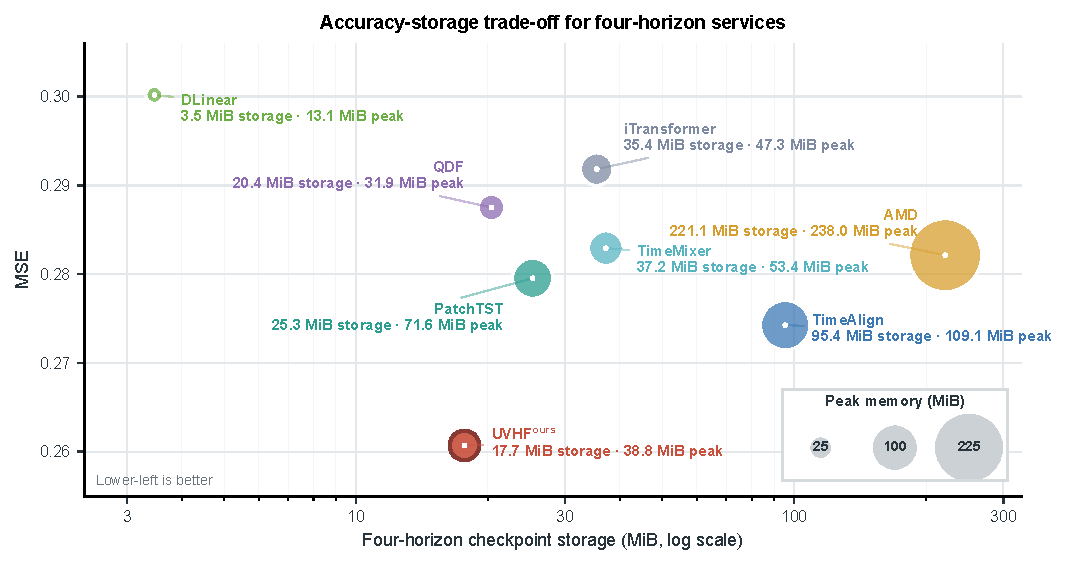
\includegraphics[width=0.90\textwidth]{figure_05_uvhf_accuracy_system_cost.pdf}
\caption{Accuracy and system cost for four-horizon forecasting. Macro MSE is plotted against total checkpoint storage, and bubble area represents peak allocated inference memory. The storage axis is logarithmic; lower-left positions indicate a more favorable trade-off.}
\label{fig:accuracy-system-cost}
\end{figure*}


As shown in Fig.~\ref{fig:accuracy-system-cost}, UVHF attains the lowest macro MSE among the eight displayed methods, at 0.261, while requiring 17.677 MiB of checkpoint storage and 38.817 MiB of peak allocated inference memory. Compared with TimeAlign, AMD, iTransformer, PatchTST and TimeMixer, the unified model reduces checkpoint storage by 30.12--92.01\% and peak memory by 18.01--83.69\%. Relative to TimeAlign in particular, UVHF lowers MSE by 4.94\%, checkpoint storage by 81.48\% and peak memory by 64.42\%.

\subsection{Component and training-objective ablations}
\label{sec:ablation}


To determine whether the individual UVHF components contribute to forecasting performance, we conduct strictly controlled ablations in which each variant is trained end to end under the same protocol. \textbf{w/o BCA} retains the Uniform-Prefix Forecasting Loss but removes the Scope-Wise Forecasting Loss and Allocation-Balance Regularizer. \textbf{w/o Target-Adaptive Allocation} replaces learned Scope Probabilities with equal non-adaptive fusion. \textbf{Shared Scope Projection} replaces the scope-specific history projections with one shared projection, whereas \textbf{Fixed Scope ($s=144$)} retains only the preregistered middle scope.

\begin{table*}[t]
\centering
\caption{Core ablation of UVHF. Each dataset entry is the mean over prediction horizons $H\in\{96,192,336,720\}$. Lower is better. Best and second-best results are shown in bold and underlined, respectively.}
\label{tab:core-ablation}
\resizebox{\textwidth}{!}{%
\begin{tabular}{lcccccccccccc}
\toprule
Variant & \multicolumn{2}{c}{ETTm1} & \multicolumn{2}{c}{ETTm2} & \multicolumn{2}{c}{ETTh1} & \multicolumn{2}{c}{ETTh2} & \multicolumn{2}{c}{Weather} & \multicolumn{2}{c}{Avg} \\
\cmidrule(lr){2-3} \cmidrule(lr){4-5} \cmidrule(lr){6-7} \cmidrule(lr){8-9} \cmidrule(lr){10-11} \cmidrule(lr){12-13}
 & MSE & MAE & MSE & MAE & MSE & MAE & MSE & MAE & MSE & MAE & MSE & MAE \\
\midrule
Full UVHF & \textbf{0.342} & \textbf{0.365} & \textbf{0.253} & \textbf{0.309} & \textbf{0.407} & \textbf{0.432} & \textbf{0.311} & \textbf{0.367} & \textbf{0.214} & \textbf{0.245} & \textbf{0.305} & \textbf{0.344} \\
\midrule
w/o BCA & 0.353 & 0.378 & \underline{0.258} & 0.315 & 0.434 & 0.450 & 0.319 & 0.375 & 0.218 & 0.250 & 0.316 & 0.354 \\
w/o Target-Adaptive Allocation & \underline{0.347} & \underline{0.369} & 0.259 & 0.317 & \underline{0.413} & 0.437 & \underline{0.315} & \underline{0.371} & \underline{0.217} & \underline{0.249} & \underline{0.310} & \underline{0.349} \\
Shared Scope Projection & 0.355 & 0.376 & \underline{0.258} & \underline{0.314} & 0.415 & \underline{0.435} & 0.325 & 0.382 & \underline{0.217} & 0.250 & 0.314 & 0.351 \\
Fixed Scope ($s=144$) & 0.351 & 0.372 & 0.263 & 0.319 & 0.428 & 0.441 & 0.318 & 0.373 & \underline{0.217} & \underline{0.249} & 0.315 & 0.351 \\
\bottomrule
\end{tabular}%
}
\end{table*}


As reported in Table~\ref{tab:core-ablation}, Full UVHF achieves a five-dataset macro MSE/MAE of 0.305/0.344 and ranks first in all 12 dataset and average metric columns. Removing BCA causes the largest aggregate decline, while equal fusion, Shared Scope Projection and Fixed Scope also increase both error metrics. Full UVHF improves MSE and MAE over every control on all five datasets.

The controlled comparisons support the utility of BCA, Target-Adaptive Scope Allocation, scope-specific projections and the multi-scope generation implemented by the MSD. Their joint design yields the strongest aggregate forecasting performance.

\subsection{Scope diversity and allocation behavior}
\label{sec:scope-behavior}


The ablation results support the contribution of the individual UVHF components to forecasting accuracy. We further examine whether the complete model exhibits the intended internal behavior. The analysis asks whether jointly trained scope lines retain distinct forecast signals and whether the Target-Adaptive Allocation Path produces diverse preferences across future regions. Region-specific forecast generation requires both properties: scope lines must avoid trajectory collapse, and allocation must vary across the future domain.

We concatenate the region-wise predictions from each scope line into its complete Scope-conditioned Forecast. Direct overlay obscures the differences among the five trajectories, so Fig.~\ref{fig:scope-allocation-behavior}b visualizes their deviations from the fused trajectory, $\mathcal F_\tau^{(s)}-\widehat y_\tau$. The profiles exhibit distinct temporal structures, with a mean pairwise absolute disagreement of 0.0812 on the normalized scale. The scope-indexed forecast field therefore retains distinct candidate signals for region-wise integration and avoids collapse to repeated trajectories.

Fig.~\ref{fig:scope-allocation-behavior}a shows how the Target-Adaptive Allocation Path combines these heterogeneous scope signals. The fused maximum-horizon forecast is coloured by the scope receiving the highest mean Scope Probability within each future region. All five scopes attain the highest weight in at least one of the eight regions, indicating that allocation avoids collapse to a fixed regional preference. Fig.~\ref{fig:scope-allocation-behavior}c displays the complete per-step Scope Probabilities, whose relative ordering varies across future steps and regions. The farthest region assigns its highest mean weight to the largest sharing scope, $s=720$, consistent with the role of broader information sharing in distal forecasting. The three panels illustrate how distinct scope signals and region-dependent soft allocation support region-specific forecast generation. These signals are fused into one shared trajectory, while prefix-based inference preserves CHPC with a maximum absolute CHPD of 0 across all 20 dataset--horizon checks.



\begin{figure*}[t]
\centering
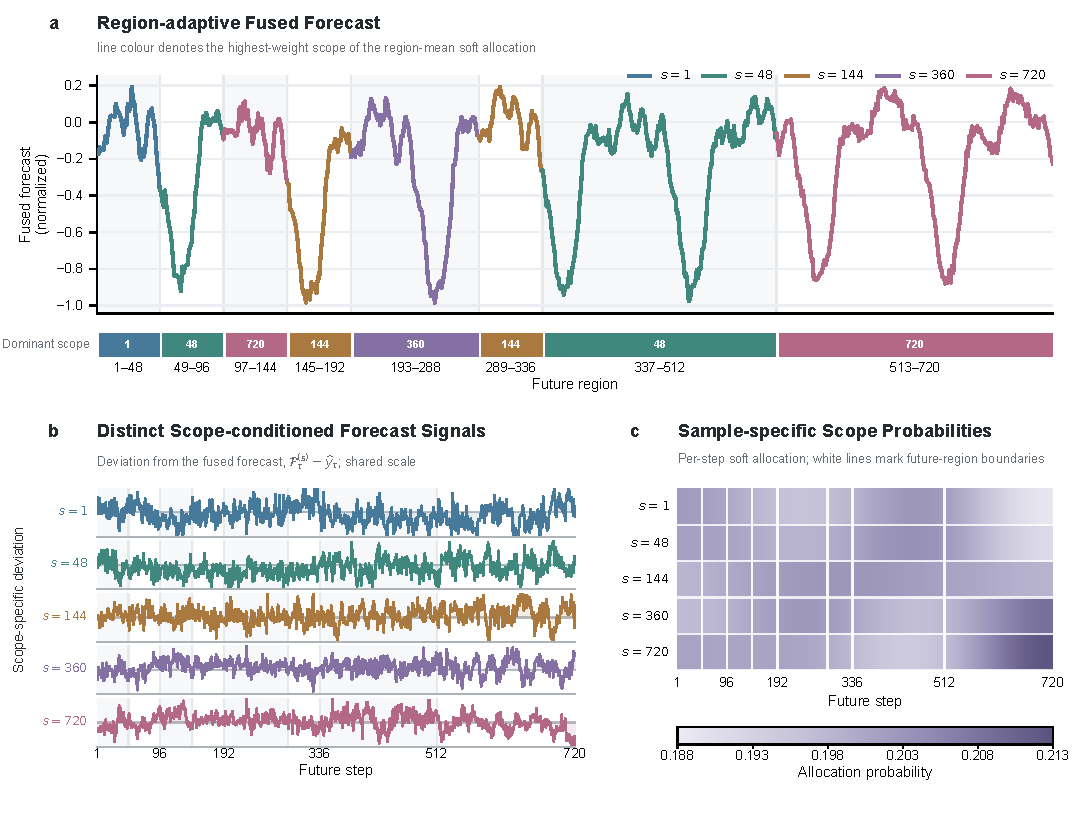
\includegraphics[width=1.00\textwidth]{figure_06_uvhf_scope_allocation_behavior.pdf}
\caption{Scope diversity and sample-specific allocation behavior in UVHF. \textbf{a}, The fused forecast; line colour and the lower strip identify the highest-weight scope after averaging Scope Probabilities within each future region. \textbf{b}, Deviations of the five Scope-conditioned Forecasts from the fused forecast on a shared scale. \textbf{c}, Per-step Scope Probabilities; white lines mark future-region boundaries.}
\label{fig:scope-allocation-behavior}
\end{figure*}


\subsection{Generalization studies}
\label{sec:generalization}


The MSD is designed as an Encoder-agnostic plug-in decoder that operates on Encoder-produced history representations. We examine this versatility using DLinear and PatchTST as representatives of lightweight linear and Transformer-based Encoders, respectively \citep{zeng2023dlinear,nie2023patchtst}. For each backbone, we replace the Original Decoder with the MSD and train the resulting UVHF instantiation end to end using BCA.



\begin{figure*}[t]
\centering
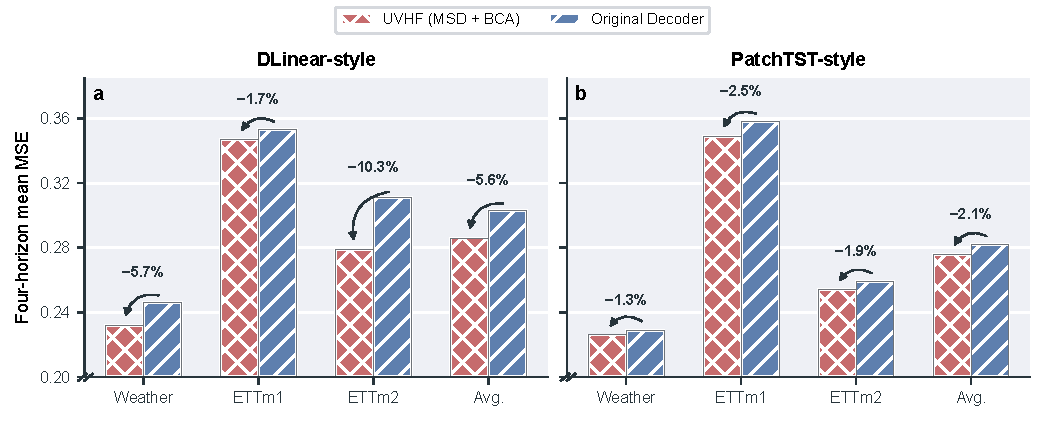
\includegraphics[width=0.90\textwidth]{figure_07_uvhf_generalization.pdf}
\caption{Generalization across two forecasting backbones. Four-horizon mean MSE is reported for \textbf{a}, DLinear and \textbf{b}, PatchTST with either the Original Decoder or UVHF (MSD trained with BCA).}
\label{fig:decoder-transfer}
\end{figure*}


As shown in Fig.~\ref{fig:decoder-transfer}, replacing the Original Decoder with the MSD and applying BCA improves forecasting performance on both example backbones. For DLinear, the replacement lowers MSE on all three datasets and reduces the macro average from 0.303 to 0.286, corresponding to an improvement of 5.61\%. PatchTST shows smaller but consistent gains, with macro MSE decreasing from 0.282 to 0.276, corresponding to an improvement of 2.13\%. Improvements with both a lightweight linear backbone and a Transformer-based backbone support the portability of the MSD and its role within UVHF.

\section{Discussion and Limitations}
\label{sec:discussion}


\textbf{Unified varied-horizon forecasting.} This task serves different request endpoints from a single prediction trajectory. Horizon-specific predictors optimize each endpoint independently and do not enforce CHPC across their overlapping outputs. UVHF maps a shared history representation and future-step coordinates to one trajectory, whose prefixes answer requests of different lengths. The experiments in Sections~\ref{sec:horizon-specific-comparison} and~\ref{sec:one-model-comparison} show that this structural consistency coexists with strong forecasting accuracy, and Fig.~\ref{fig:accuracy-system-cost} demonstrates the deployment benefit of consolidating all horizon requests into one checkpoint.

\textbf{Output-side multi-scope generation.} Existing multi-scale encoders extract and combine historical dependencies at multiple input resolutions, where scale describes the granularity of history representation before decoding \citep{challu2023nhits,chen2024pathformer,wang2024timemixer}. The MSD introduces a distinct output-side formulation in which candidate forecasts reuse history-conditioned latent states over different contiguous future extents. Each scope therefore specifies the sharing granularity of forecast generation, shifting multi-scale modeling from history representation to future construction. Evidence from the scope-wise ablations, the future-region analysis in Section 3 and the Fig.~\ref{fig:scope-allocation-behavior} diagnostics indicates that different future regions can benefit from different sharing extents. Target-Adaptive Allocation assigns step-specific preferences across these candidate forecast signals. Multi-scale encoders and the MSD address separate yet complementary stages of the forecasting pipeline. Multi-scale encoders organize historical evidence, while the MSD converts the resulting shared representation into forecasts at multiple future-sharing granularities.

\textbf{Methodological limitations.} The current formulation relies on a finite set of pre-specified contiguous scopes and future regions. This assumption may be restrictive when useful sharing patterns change at irregular locations, motivating data-adaptive region partitioning. Interactions among region forecasts are mediated through the shared History State and Future Coordinate. A dedicated cross-region forecasting mechanism could model dependencies that evolve across the future domain more explicitly. Multiple scope branches also increase decoder-side computation compared with a single-scope head, although shared encoding and unified serving reduce duplicated computation and storage. Future work should examine adaptive partitioning, cross-region interactions and more efficient multi-scope generation.

\section{Conclusion}
\label{sec:conclusion}


This work reframes multi-horizon service as the construction of one coherent future trajectory, with request endpoints exposed through nested prefixes. Within this formulation, CHPC defines the required cross-horizon coherence, and output-side sharing granularity becomes an explicit dimension of forecast generation. UVHF realizes this principle through an MSD that constructs Scope-conditioned Forecasts across multiple sharing extents and integrates them through Target-Adaptive Allocation. BCA supplies balanced supervision to the jointly optimized scope lines. The resulting framework combines region-sensitive forecast generation with prefix-consistent inference in a single horizon-agnostic model.

Across seven multivariate benchmarks, UVHF achieved state-of-the-art aggregate accuracy among the evaluated methods while consolidating every supported horizon into one model. Its advantage persisted under a common one-model-all-horizons workflow, and controlled ablations and two-backbone studies supported component utility and MSD portability. These findings connect prefix-consistent serving with strong forecasting accuracy and efficient model consolidation in one framework. They also position output-side sharing granularity as a productive design axis for unified time-series forecasting.
%% END INLINED UVHF MAIN TEXT

\section*{CRediT authorship contribution statement}
\indent \textbf{Chenhao Ying:} Writing -- original draft, Writing - review \& editing, Visualization, Validation, Supervision, Software, Resources, Project administration, Methodology, Investigation. \textbf{Jiangang Lu:} Writing - review \& editing, Conceptualization.

\section*{Declaration of Competing Interest}
\indent The authors declare that they have no known competing financial interests or personal relationships that could have appeared to influence the work reported in this paper.

\section*{Data availability}
Data will be made available on request.

\section*{Acknowledgments}
This work was supported in part by the National Natural Science Foundation of China under Grant 62293504, 62293500, and in part by Zhejiang Province Science and Technology Plan Project under Grant 2025C01091.

\appendix
\renewcommand*{\theHtable}{appendix.\Alph{section}.\arabic{table}}
\renewcommand*{\theHfigure}{appendix.\Alph{section}.\arabic{figure}}

%% BEGIN INLINED UVHF APPENDICES
\setcounter{table}{0}
\setcounter{figure}{0}
\section{Experiment Details}
\label{app:experiment-details}


\subsection{Metric Details}


We use mean squared error (MSE) and mean absolute error (MAE) to evaluate forecasting accuracy. Given the ground-truth values $y_i$ and their predictions $\widehat y_i$, the two metrics are defined as

\begin{equation}
\operatorname{MSE}
=
\frac{1}{N}
\sum_{i=1}^{N}
\left(y_i-\widehat y_i\right)^2,
\qquad
\operatorname{MAE}
=
\frac{1}{N}
\sum_{i=1}^{N}
\left|y_i-\widehat y_i\right|,
\end{equation}


where $N$ is the total number of scalar predictions over all evaluation windows, forecast steps and variables for the requested horizon. Lower MSE and MAE indicate more accurate forecasts.

\subsection{Datasets}


We evaluate UVHF on seven widely used multivariate time-series forecasting datasets spanning electricity transformers, electricity consumption, meteorology and solar generation. These benchmarks differ substantially in variable dimension, sampling frequency and temporal dynamics. Table~\ref{tab:dataset-statistics} summarizes their basic statistics.

\begin{enumerate}
\item \textbf{ETT (Electricity Transformer Temperature)} records seven load and temperature factors from two electricity transformers in two regions of China between 2016 and 2018 \citep{zhou2021informer}. We use its four standard subsets: ETTh1 and ETTh2 are sampled hourly, whereas ETTm1 and ETTm2 are sampled every 15 minutes.
\item \textbf{Electricity (ECL)}\footnote{\url{https://archive.ics.uci.edu/dataset/321}} records the hourly electricity consumption of 321 clients from 2012 to 2014 and is provided by the UCI Machine Learning Repository.
\item \textbf{Weather}\footnote{\url{https://www.bgc-jena.mpg.de/wetter/}} is collected by the Beutenberg Weather Station at the Max Planck Institute for Biogeochemistry in Jena, Germany. It contains 21 meteorological indicators sampled every 10 minutes during 2020 \citep{wu2023timesnet}.
\item \textbf{Solar} contains solar-power measurements collected every 10 minutes from 137 photovoltaic plants in Alabama during 2006 \citep{lai2018lstnet}.
\end{enumerate}

\begin{table*}[t]
\centering
\scriptsize
\setlength{\tabcolsep}{4pt}
\caption{Dataset Statistics.}
\label{tab:dataset-statistics}
\begin{tabular}{lcccc}
\toprule
Dataset & Variables & Sampling Frequency & Dataset Size & Domain \\
\midrule
ETTh1 & 7 & 1 h & (8545, 2881, 2881) & Electricity \\
ETTh2 & 7 & 1 h & (8545, 2881, 2881) & Electricity \\
ETTm1 & 7 & 15 min & (34465, 11521, 11521) & Electricity \\
ETTm2 & 7 & 15 min & (34465, 11521, 11521) & Electricity \\
ECL & 321 & 1 h & (18317, 2633, 5261) & Electricity \\
Weather & 21 & 10 min & (36792, 5271, 10540) & Weather \\
Solar & 137 & 10 min & (36601, 5161, 10417) & Solar energy \\
\bottomrule
\end{tabular}
\end{table*}


Dataset Size is reported as (Train, Validation, Test). The ETT datasets follow their standard fixed chronological splits, whereas Weather, ECL and Solar use chronological 70/10/20 splits. The scaler is fitted exclusively on the training segment. All datasets are evaluated at prediction lengths $H\in\{96,192,336,720\}$.

\subsection{Implementation Details}


The local experiments are implemented in Python 3.12.13 and PyTorch 2.9.0 with CUDA 12.8. Each training run uses one NVIDIA GeForce RTX 3090 GPU. UVHF is trained from scratch with BCA using AdamW and a cosine learning-rate schedule \citep{loshchilov2019adamw,loshchilov2017sgdr}. Table~\ref{tab:training-settings} reports the dataset-specific optimization settings, and Table~\ref{tab:model-settings} lists the corresponding Encoder interface and UVHF configuration.

\begin{table*}[t]
\centering
\scriptsize
\setlength{\tabcolsep}{4pt}
\caption{Training and Evaluation Settings.}
\label{tab:training-settings}
\begin{tabular}{lcccccc}
\toprule
Dataset & Max Length & Initial LR & Batch & Grad. Accum. & Max epochs & Patience \\
\midrule
ETTh1 & 720 & $3\times10^{-4}$ & 32 & 1 & 45 & 10 \\
ETTh2 & 720 & $5\times10^{-4}$ & 32 & 1 & 30 & 7 \\
ETTm1 & 720 & $1\times10^{-4}$ & 16 & 2 & 30 & 7 \\
ETTm2 & 720 & $5\times10^{-5}$ & 16 & 2 & 60 & 12 \\
Weather & 720 & $2\times10^{-5}$ & 32 & 1 & 120 & 24 \\
ECL & 720 & $5\times10^{-4}$ & 4 & 8 & 30 & 7 \\
Solar & 720 & $3\times10^{-4}$ & 16 & 2 & 45 & 10 \\
\bottomrule
\end{tabular}
\end{table*}


Gradient Accumulation Steps denotes the number of mini-batches whose gradients are accumulated before one optimizer update; the effective batch size is therefore the batch size multiplied by this value. All runs use seed 2021. The checkpoint with the lowest validation mean MSE over $H\in\{96,192,336,720\}$ is retained and serves all four forecasting requests. Weight decay is $0.01$ except for ETTm2, where it is $0.001$, and early stopping uses zero minimum improvement.

\begin{table*}[t]
\centering
\scriptsize
\setlength{\tabcolsep}{4pt}
\caption{UVHF Configuration.}
\label{tab:model-settings}
\resizebox{\textwidth}{!}{%
\begin{tabular}{lccccccccc}
\toprule
Dataset & Scope set & Mode rank & Patch number & $d_{\mathrm{model}}$ & $d_{\mathrm{ff}}$ & Dropout & Weight decay & $\lambda_{\mathrm{scope}}$ & $\lambda_{\mathrm{balance}}^{\max}/u_{\mathrm{ramp}}$ \\
\midrule
ETTh1 & $\{1,48,144,360,720\}$ & 109 & 24 & 32 & 32 & 0.1 & 0.01 & 1.0 & 0.1 / 0.25 \\
ETTh2 & $\{1,48,144,360,720\}$ & 116 & 12 & 64 & 128 & 0.1 & 0.01 & 1.0 & 0.1 / 0.25 \\
ETTm1 & $\{1,48,144,360,720\}$ & 116 & 1 & 128 & 256 & 0.9 & 0.01 & 1.0 & 0.1 / 0.25 \\
ETTm2 & $\{1,48,144,360,720\}$ & 64 & 6 & 128 & 128 & 0.2 & 0.001 & 1.0 & 0.1 / 0.25 \\
Weather & $\{1,48,144,360,720\}$ & 116 & 19 & 64 & 128 & 0.0 & 0.01 & 1.0 & 0.1 / 0.25 \\
ECL & $\{1,48,144,360,720\}$ & 64 & 1 & 256 & 1,024 & 0.3 & 0.01 & 1.0 & 0.1 / 0.25 \\
Solar & $\{1,48,144,360,720\}$ & 128 & 4 & 256 & 256 & 0.3 & 0.01 & 1.0 & 0.1 / 0.25 \\
\bottomrule
\end{tabular}%
}
\end{table*}


The scope set and BCA coefficients are shared across datasets.
Specifically,

\begin{equation}
\lambda_{\mathrm{scope}}=1,
\qquad
\lambda_{\mathrm{balance}}(u)
=
\lambda_{\mathrm{balance}}^{\max}
\min\!\left(u/u_{\mathrm{ramp}},1\right),
\end{equation}

where $u\in[0,1]$ denotes normalized optimizer progress, $\lambda_{\mathrm{balance}}^{\max}$ is the maximum balance weight and $u_{\mathrm{ramp}}$ is the progress at which this weight is reached. We use $\lambda_{\mathrm{balance}}^{\max}=0.1$ and $u_{\mathrm{ramp}}=0.25$ for every dataset.

\setcounter{table}{0}
\setcounter{figure}{0}
\section{Full Results}
\label{app:full-results}


Tables~\ref{tab:appendix-horizon-specific} and~\ref{tab:appendix-one-model} report the complete horizon-wise MSE and MAE results underlying Sections~\ref{sec:horizon-specific-comparison} and~\ref{sec:one-model-comparison}. Table~\ref{tab:appendix-horizon-specific} compares UVHF with horizon-specific baselines, while Table~\ref{tab:appendix-one-model} evaluates every method under the one-model-all-horizons workflow. The main text reports the corresponding four-horizon dataset averages.

% Required packages: booktabs, multirow, graphicx, xcolor
\begin{table}[H]
\centering
\scriptsize
\setlength{\tabcolsep}{1.2pt}
\resizebox{\textwidth}{!}{%
\begin{tabular}{cc|cc|cc|cc|cc|cc|cc|cc|cc|cc|cc|cc}
\toprule
Dataset & H & \multicolumn{2}{c}{\shortstack{UVHF\\(Ours)}} & \multicolumn{2}{c}{\shortstack{TimeAlign\\(2026)}} & \multicolumn{2}{c}{\shortstack{QDF\\(2026)}} & \multicolumn{2}{c}{\shortstack{AMD\\(2025)}} & \multicolumn{2}{c}{\shortstack{SimpleTM\\(2025)}} & \multicolumn{2}{c}{\shortstack{TVNet\\(2025)}} & \multicolumn{2}{c}{\shortstack{iTransformer\\(2024)}} & \multicolumn{2}{c}{\shortstack{TimeMixer\\(2024)}} & \multicolumn{2}{c}{\shortstack{ModernTCN\\(2024)}} & \multicolumn{2}{c}{\shortstack{PatchTST\\(2023)}} & \multicolumn{2}{c}{\shortstack{DLinear\\(2023)}} \\
 &  & MSE & MAE & MSE & MAE & MSE & MAE & MSE & MAE & MSE & MAE & MSE & MAE & MSE & MAE & MSE & MAE & MSE & MAE & MSE & MAE & MSE & MAE \\
\midrule
\multirow{5}{*}{ETTm1} & 96 & \textcolor{red}{\textbf{0.265}} & \textcolor{red}{\textbf{0.326}} & \textcolor{blue}{\underline{0.280}} & \textcolor{blue}{\underline{0.331}} & 0.283 & 0.336 & 0.289 & 0.343 & 0.325 & 0.363 & 0.288 & 0.343 & 0.300 & 0.353 & 0.293 & 0.345 & 0.292 & 0.346 & 0.293 & 0.346 & 0.300 & 0.345 \\
 & 192 & \textcolor{red}{\textbf{0.304}} & \textcolor{red}{\textbf{0.349}} & \textcolor{blue}{\underline{0.323}} & \textcolor{blue}{\underline{0.357}} & 0.336 & 0.369 & 0.329 & 0.366 & 0.361 & 0.381 & 0.326 & 0.367 & 0.345 & 0.382 & 0.335 & 0.372 & 0.332 & 0.368 & 0.333 & 0.370 & 0.336 & 0.366 \\
 & 336 & \textcolor{red}{\textbf{0.343}} & \textcolor{blue}{\underline{0.371}} & \textcolor{blue}{\underline{0.352}} & 0.376 & 0.369 & 0.390 & 0.365 & 0.386 & 0.391 & 0.404 & 0.365 & 0.391 & 0.374 & 0.398 & 0.368 & 0.386 & 0.365 & 0.391 & 0.369 & \textcolor{red}{\textbf{0.369}} & 0.367 & 0.386 \\
 & 720 & \textcolor{red}{\textbf{0.404}} & \textcolor{red}{\textbf{0.405}} & \textcolor{blue}{\underline{0.408}} & \textcolor{blue}{\underline{0.409}} & 0.423 & 0.424 & 0.423 & 0.417 & 0.454 & 0.438 & 0.412 & 0.413 & 0.429 & 0.430 & 0.426 & 0.417 & 0.416 & 0.417 & 0.416 & 0.420 & 0.419 & 0.416 \\
\cmidrule(lr){2-24}
 & Avg. & \textcolor{red}{\textbf{0.329}} & \textcolor{red}{\textbf{0.363}} & \textcolor{blue}{\underline{0.341}} & \textcolor{blue}{\underline{0.368}} & 0.353 & 0.380 & 0.351 & 0.378 & 0.383 & 0.396 & 0.348 & 0.379 & 0.362 & 0.391 & 0.356 & 0.380 & 0.351 & 0.381 & 0.353 & 0.376 & 0.356 & 0.378 \\
\midrule
\multirow{5}{*}{ETTm2} & 96 & \textcolor{blue}{\underline{0.159}} & \textcolor{red}{\textbf{0.242}} & \textcolor{red}{\textbf{0.157}} & \textcolor{blue}{\underline{0.244}} & 0.164 & 0.253 & 0.168 & 0.258 & 0.175 & 0.258 & 0.161 & 0.254 & 0.175 & 0.266 & 0.165 & 0.256 & 0.166 & 0.256 & 0.166 & 0.256 & 0.164 & 0.255 \\
 & 192 & \textcolor{blue}{\underline{0.218}} & \textcolor{blue}{\underline{0.285}} & \textcolor{red}{\textbf{0.210}} & \textcolor{red}{\textbf{0.280}} & \textcolor{blue}{\underline{0.218}} & 0.291 & 0.221 & 0.295 & 0.240 & 0.301 & 0.220 & 0.293 & 0.242 & 0.312 & 0.225 & 0.298 & 0.222 & 0.293 & 0.223 & 0.296 & 0.224 & 0.304 \\
 & 336 & \textcolor{blue}{\underline{0.270}} & \textcolor{blue}{\underline{0.318}} & \textcolor{red}{\textbf{0.265}} & \textcolor{blue}{\underline{0.318}} & 0.282 & 0.330 & \textcolor{blue}{\underline{0.270}} & 0.327 & 0.305 & 0.342 & 0.272 & \textcolor{red}{\textbf{0.316}} & 0.282 & 0.340 & 0.277 & 0.332 & 0.272 & 0.324 & 0.274 & 0.329 & 0.277 & 0.337 \\
 & 720 & \textcolor{red}{\textbf{0.343}} & \textcolor{red}{\textbf{0.371}} & \textcolor{blue}{\underline{0.346}} & \textcolor{blue}{\underline{0.374}} & 0.364 & 0.385 & 0.355 & 0.381 & 0.401 & 0.399 & 0.349 & 0.379 & 0.378 & 0.398 & 0.360 & 0.387 & 0.351 & 0.381 & 0.362 & 0.385 & 0.371 & 0.401 \\
\cmidrule(lr){2-24}
 & Avg. & \textcolor{blue}{\underline{0.248}} & \textcolor{red}{\textbf{0.304}} & \textcolor{red}{\textbf{0.245}} & \textcolor{red}{\textbf{0.304}} & 0.257 & 0.315 & 0.254 & 0.315 & 0.280 & 0.325 & 0.251 & \textcolor{blue}{\underline{0.311}} & 0.269 & 0.329 & 0.257 & 0.318 & 0.253 & 0.314 & 0.256 & 0.317 & 0.259 & 0.324 \\
\midrule
\multirow{5}{*}{ETTh1} & 96 & \textcolor{red}{\textbf{0.348}} & \textcolor{red}{\textbf{0.386}} & 0.380 & 0.407 & 0.370 & 0.394 & 0.371 & 0.399 & \textcolor{blue}{\underline{0.367}} & \textcolor{blue}{\underline{0.393}} & 0.371 & 0.408 & 0.386 & 0.405 & 0.372 & 0.401 & 0.368 & 0.394 & 0.377 & 0.397 & 0.379 & 0.403 \\
 & 192 & \textcolor{red}{\textbf{0.377}} & \textcolor{red}{\textbf{0.403}} & 0.406 & 0.419 & 0.422 & 0.427 & 0.403 & 0.420 & 0.429 & 0.427 & \textcolor{blue}{\underline{0.398}} & \textcolor{blue}{\underline{0.409}} & 0.424 & 0.440 & 0.413 & 0.430 & 0.405 & 0.413 & 0.409 & 0.428 & 0.408 & 0.419 \\
 & 336 & \textcolor{blue}{\underline{0.393}} & 0.414 & 0.427 & 0.432 & 0.464 & 0.455 & 0.423 & 0.432 & 0.447 & 0.445 & 0.401 & \textcolor{red}{\textbf{0.409}} & 0.449 & 0.460 & 0.438 & 0.450 & \textcolor{red}{\textbf{0.391}} & \textcolor{blue}{\underline{0.412}} & 0.431 & 0.444 & 0.440 & 0.440 \\
 & 720 & \textcolor{red}{\textbf{0.443}} & \textcolor{red}{\textbf{0.458}} & 0.459 & 0.464 & 0.499 & 0.493 & 0.452 & 0.461 & 0.470 & 0.465 & 0.458 & \textcolor{blue}{\underline{0.459}} & 0.495 & 0.487 & 0.486 & 0.484 & \textcolor{blue}{\underline{0.450}} & 0.461 & 0.457 & 0.477 & 0.471 & 0.493 \\
\cmidrule(lr){2-24}
 & Avg. & \textcolor{red}{\textbf{0.390}} & \textcolor{red}{\textbf{0.415}} & 0.418 & 0.431 & 0.439 & 0.442 & 0.412 & 0.428 & 0.428 & 0.433 & 0.407 & 0.421 & 0.439 & 0.448 & 0.427 & 0.441 & \textcolor{blue}{\underline{0.404}} & \textcolor{blue}{\underline{0.420}} & 0.419 & 0.437 & 0.425 & 0.439 \\
\midrule
\multirow{5}{*}{ETTh2} & 96 & \textcolor{red}{\textbf{0.241}} & \textcolor{red}{\textbf{0.314}} & 0.270 & 0.331 & 0.283 & 0.342 & 0.279 & 0.343 & 0.285 & 0.342 & \textcolor{blue}{\underline{0.263}} & \textcolor{blue}{\underline{0.329}} & 0.297 & 0.348 & 0.281 & 0.351 & \textcolor{blue}{\underline{0.263}} & 0.332 & 0.274 & 0.337 & 0.289 & 0.353 \\
 & 192 & \textcolor{red}{\textbf{0.282}} & \textcolor{red}{\textbf{0.345}} & 0.334 & 0.374 & 0.359 & 0.391 & 0.363 & 0.397 & 0.357 & 0.387 & \textcolor{blue}{\underline{0.319}} & \textcolor{blue}{\underline{0.372}} & 0.371 & 0.403 & 0.349 & 0.387 & 0.320 & 0.374 & 0.348 & 0.384 & 0.383 & 0.418 \\
 & 336 & \textcolor{red}{\textbf{0.310}} & \textcolor{red}{\textbf{0.369}} & 0.376 & 0.405 & 0.361 & 0.401 & 0.381 & 0.419 & 0.369 & 0.402 & \textcolor{blue}{\underline{0.311}} & \textcolor{blue}{\underline{0.373}} & 0.404 & 0.428 & 0.366 & 0.413 & 0.313 & 0.376 & 0.377 & 0.416 & 0.448 & 0.465 \\
 & 720 & \textcolor{red}{\textbf{0.392}} & \textcolor{red}{\textbf{0.429}} & 0.406 & 0.436 & 0.407 & 0.440 & 0.442 & 0.467 & 0.414 & 0.436 & \textcolor{blue}{\underline{0.401}} & 0.434 & 0.424 & 0.444 & \textcolor{blue}{\underline{0.401}} & 0.436 & \textcolor{red}{\textbf{0.392}} & \textcolor{blue}{\underline{0.433}} & 0.406 & 0.441 & 0.605 & 0.551 \\
\cmidrule(lr){2-24}
 & Avg. & \textcolor{red}{\textbf{0.306}} & \textcolor{red}{\textbf{0.364}} & 0.347 & 0.387 & 0.353 & 0.394 & 0.366 & 0.406 & 0.356 & 0.392 & 0.324 & \textcolor{blue}{\underline{0.377}} & 0.374 & 0.406 & 0.349 & 0.397 & \textcolor{blue}{\underline{0.322}} & 0.379 & 0.351 & 0.395 & 0.431 & 0.447 \\
\midrule
\multirow{5}{*}{Weather} & 96 & \textcolor{red}{\textbf{0.140}} & \textcolor{red}{\textbf{0.180}} & \textcolor{blue}{\underline{0.143}} & \textcolor{blue}{\underline{0.182}} & 0.152 & 0.202 & 0.148 & 0.203 & 0.157 & 0.204 & 0.147 & 0.198 & 0.159 & 0.208 & 0.147 & 0.198 & 0.149 & 0.200 & 0.149 & 0.198 & 0.170 & 0.230 \\
 & 192 & \textcolor{red}{\textbf{0.181}} & \textcolor{red}{\textbf{0.223}} & \textcolor{blue}{\underline{0.185}} & \textcolor{blue}{\underline{0.224}} & 0.205 & 0.251 & 0.193 & 0.243 & 0.205 & 0.248 & 0.194 & 0.238 & 0.200 & 0.248 & 0.192 & 0.243 & 0.196 & 0.245 & 0.194 & 0.241 & 0.216 & 0.273 \\
 & 336 & \textcolor{red}{\textbf{0.231}} & \textcolor{red}{\textbf{0.263}} & \textcolor{blue}{\underline{0.235}} & \textcolor{red}{\textbf{0.263}} & 0.248 & 0.282 & 0.242 & 0.281 & 0.264 & 0.291 & \textcolor{blue}{\underline{0.235}} & \textcolor{blue}{\underline{0.277}} & 0.253 & 0.289 & 0.247 & 0.284 & 0.238 & \textcolor{blue}{\underline{0.277}} & 0.245 & 0.282 & 0.258 & 0.307 \\
 & 720 & \textcolor{red}{\textbf{0.302}} & \textcolor{red}{\textbf{0.313}} & \textcolor{blue}{\underline{0.308}} & \textcolor{blue}{\underline{0.319}} & 0.341 & 0.351 & 0.315 & 0.332 & 0.346 & 0.344 & \textcolor{blue}{\underline{0.308}} & 0.331 & 0.321 & 0.338 & 0.318 & 0.330 & 0.314 & 0.334 & 0.314 & 0.334 & 0.323 & 0.362 \\
\cmidrule(lr){2-24}
 & Avg. & \textcolor{red}{\textbf{0.214}} & \textcolor{red}{\textbf{0.245}} & \textcolor{blue}{\underline{0.218}} & \textcolor{blue}{\underline{0.247}} & 0.237 & 0.271 & 0.225 & 0.265 & 0.243 & 0.271 & 0.221 & 0.261 & 0.233 & 0.271 & 0.226 & 0.264 & 0.224 & 0.264 & 0.226 & 0.264 & 0.242 & 0.293 \\
\midrule
\multirow{5}{*}{ECL} & 96 & \textcolor{red}{\textbf{0.116}} & \textcolor{red}{\textbf{0.213}} & 0.128 & \textcolor{blue}{\underline{0.218}} & \textcolor{blue}{\underline{0.127}} & 0.222 & 0.131 & 0.228 & 0.143 & 0.237 & 0.142 & 0.223 & 0.138 & 0.237 & 0.142 & 0.247 & 0.129 & 0.226 & 0.129 & 0.222 & 0.140 & 0.237 \\
 & 192 & \textcolor{red}{\textbf{0.136}} & \textcolor{red}{\textbf{0.231}} & 0.145 & \textcolor{blue}{\underline{0.235}} & 0.151 & 0.244 & 0.151 & 0.244 & 0.151 & 0.248 & 0.165 & 0.241 & 0.157 & 0.256 & 0.168 & 0.269 & \textcolor{blue}{\underline{0.143}} & 0.239 & 0.147 & 0.240 & 0.152 & 0.249 \\
 & 336 & \textcolor{red}{\textbf{0.157}} & \textcolor{red}{\textbf{0.251}} & 0.162 & \textcolor{red}{\textbf{0.251}} & 0.167 & 0.260 & 0.167 & 0.262 & 0.176 & 0.269 & 0.164 & 0.269 & 0.167 & 0.264 & 0.171 & 0.260 & \textcolor{blue}{\underline{0.161}} & \textcolor{blue}{\underline{0.259}} & 0.163 & \textcolor{blue}{\underline{0.259}} & 0.170 & 0.267 \\
 & 720 & 0.195 & \textcolor{blue}{\underline{0.280}} & \textcolor{red}{\textbf{0.190}} & \textcolor{red}{\textbf{0.278}} & 0.223 & 0.314 & 0.200 & 0.292 & 0.201 & 0.293 & \textcolor{red}{\textbf{0.190}} & 0.284 & 0.194 & 0.286 & 0.209 & 0.313 & \textcolor{blue}{\underline{0.191}} & 0.286 & 0.197 & 0.290 & 0.203 & 0.301 \\
\cmidrule(lr){2-24}
 & Avg. & \textcolor{red}{\textbf{0.151}} & \textcolor{red}{\textbf{0.244}} & \textcolor{blue}{\underline{0.156}} & \textcolor{blue}{\underline{0.246}} & 0.167 & 0.260 & 0.162 & 0.257 & 0.168 & 0.262 & 0.165 & 0.254 & 0.164 & 0.261 & 0.173 & 0.272 & \textcolor{blue}{\underline{0.156}} & 0.253 & 0.159 & 0.253 & 0.166 & 0.264 \\
\midrule
\multirow{5}{*}{Solar} & 96 & \textcolor{red}{\textbf{0.166}} & \textcolor{red}{\textbf{0.195}} & 0.182 & \textcolor{blue}{\underline{0.205}} & 0.193 & 0.232 & 0.188 & 0.235 & \textcolor{blue}{\underline{0.169}} & 0.229 & 0.204 & 0.260 & 0.188 & 0.232 & 0.179 & 0.232 & 0.202 & 0.263 & 0.178 & 0.229 & 0.197 & 0.210 \\
 & 192 & \textcolor{red}{\textbf{0.185}} & \textcolor{red}{\textbf{0.206}} & 0.198 & \textcolor{blue}{\underline{0.217}} & 0.207 & 0.261 & 0.203 & 0.246 & \textcolor{blue}{\underline{0.189}} & 0.252 & 0.227 & 0.272 & 0.193 & 0.248 & 0.201 & 0.259 & 0.223 & 0.279 & \textcolor{blue}{\underline{0.189}} & 0.246 & 0.218 & 0.222 \\
 & 336 & \textcolor{blue}{\underline{0.195}} & \textcolor{red}{\textbf{0.213}} & 0.203 & \textcolor{blue}{\underline{0.222}} & 0.210 & 0.263 & 0.213 & 0.252 & 0.199 & 0.262 & 0.241 & 0.288 & 0.203 & 0.249 & \textcolor{red}{\textbf{0.190}} & 0.256 & 0.241 & 0.292 & 0.198 & 0.249 & 0.234 & 0.231 \\
 & 720 & 0.204 & \textcolor{red}{\textbf{0.218}} & \textcolor{red}{\textbf{0.201}} & \textcolor{blue}{\underline{0.223}} & 0.223 & 0.278 & 0.215 & 0.257 & 0.207 & 0.259 & 0.242 & 0.287 & 0.223 & 0.261 & \textcolor{blue}{\underline{0.203}} & 0.261 & 0.247 & 0.292 & 0.209 & 0.256 & 0.243 & 0.241 \\
\cmidrule(lr){2-24}
 & Avg. & \textcolor{red}{\textbf{0.188}} & \textcolor{red}{\textbf{0.208}} & 0.196 & \textcolor{blue}{\underline{0.217}} & 0.208 & 0.258 & 0.205 & 0.248 & \textcolor{blue}{\underline{0.191}} & 0.251 & 0.229 & 0.277 & 0.202 & 0.248 & 0.193 & 0.252 & 0.228 & 0.282 & 0.194 & 0.245 & 0.223 & 0.226 \\
\bottomrule
\end{tabular}%
}
\caption{Full results for the horizon-specific comparison. MSE and MAE are reported for $H\in\{96,192,336,720\}$ and averaged over the four horizons. The best and second-best values are highlighted in bold and underlined, respectively.}
\label{tab:appendix-horizon-specific}
\end{table}



\clearpage
% Required packages: booktabs, multirow, graphicx, xcolor
\begin{table}[H]
\centering
\scriptsize
\setlength{\tabcolsep}{1.2pt}
\resizebox{\textwidth}{!}{%
\begin{tabular}{cc|cc|cc|cc|cc|cc|cc|cc|cc}
\toprule
Dataset & H & \multicolumn{2}{c}{UVHF (Ours)} & \multicolumn{2}{c}{TimeAlign (2026)} & \multicolumn{2}{c}{QDF (2026)} & \multicolumn{2}{c}{AMD (2025)} & \multicolumn{2}{c}{SimpleTM (2025)} & \multicolumn{2}{c}{iTransformer (2024b)} & \multicolumn{2}{c}{PatchTST (2023)} & \multicolumn{2}{c}{DLinear (2023)} \\
 &  & MSE & MAE & MSE & MAE & MSE & MAE & MSE & MAE & MSE & MAE & MSE & MAE & MSE & MAE & MSE & MAE \\
\midrule
\multirow{5}{*}{ETTm1} & 96 & \textcolor{red}{\textbf{0.265}} & \textcolor{red}{\textbf{0.326}} & \textcolor{blue}{\underline{0.290}} & \textcolor{blue}{\underline{0.338}} & 0.292 & 0.348 & 0.294 & 0.348 & 0.326 & 0.368 & 0.346 & 0.382 & 0.298 & 0.350 & 0.301 & 0.346 \\
 & 192 & \textcolor{red}{\textbf{0.304}} & \textcolor{red}{\textbf{0.349}} & \textcolor{blue}{\underline{0.325}} & \textcolor{blue}{\underline{0.358}} & 0.330 & 0.371 & 0.333 & 0.368 & 0.362 & 0.385 & 0.384 & 0.399 & 0.335 & 0.372 & 0.336 & 0.367 \\
 & 336 & \textcolor{red}{\textbf{0.343}} & \textcolor{red}{\textbf{0.371}} & \textcolor{blue}{\underline{0.355}} & \textcolor{blue}{\underline{0.378}} & 0.364 & 0.391 & 0.366 & 0.387 & 0.392 & 0.406 & 0.418 & 0.420 & 0.367 & 0.392 & 0.371 & 0.387 \\
 & 720 & \textcolor{red}{\textbf{0.404}} & \textcolor{red}{\textbf{0.405}} & \textcolor{blue}{\underline{0.408}} & \textcolor{blue}{\underline{0.409}} & 0.423 & 0.424 & 0.423 & 0.417 & 0.454 & 0.438 & 0.487 & 0.456 & 0.415 & 0.421 & 0.427 & 0.423 \\
\cmidrule(lr){2-18}
 & Avg. & \textcolor{red}{\textbf{0.329}} & \textcolor{red}{\textbf{0.363}} & \textcolor{blue}{\underline{0.345}} & \textcolor{blue}{\underline{0.371}} & 0.352 & 0.384 & 0.354 & 0.380 & 0.384 & 0.399 & 0.409 & 0.415 & 0.354 & 0.384 & 0.359 & 0.381 \\
\midrule
\multirow{5}{*}{ETTm2} & 96 & \textcolor{red}{\textbf{0.159}} & \textcolor{red}{\textbf{0.242}} & 0.168 & \textcolor{blue}{\underline{0.253}} & \textcolor{blue}{\underline{0.165}} & 0.255 & 0.170 & 0.260 & 0.186 & 0.270 & 0.190 & 0.277 & 0.169 & 0.258 & 0.189 & 0.289 \\
 & 192 & \textcolor{blue}{\underline{0.218}} & \textcolor{red}{\textbf{0.285}} & \textcolor{red}{\textbf{0.216}} & \textcolor{blue}{\underline{0.286}} & 0.223 & 0.294 & 0.222 & 0.295 & 0.247 & 0.308 & 0.253 & 0.315 & 0.223 & 0.295 & 0.256 & 0.339 \\
 & 336 & \textcolor{blue}{\underline{0.270}} & \textcolor{red}{\textbf{0.318}} & \textcolor{red}{\textbf{0.268}} & \textcolor{blue}{\underline{0.320}} & 0.276 & 0.330 & 0.271 & 0.327 & 0.305 & 0.344 & 0.318 & 0.354 & 0.275 & 0.329 & 0.320 & 0.381 \\
 & 720 & \textcolor{red}{\textbf{0.343}} & \textcolor{red}{\textbf{0.371}} & \textcolor{blue}{\underline{0.346}} & \textcolor{blue}{\underline{0.374}} & 0.364 & 0.385 & 0.355 & 0.381 & 0.401 & 0.399 & 0.416 & 0.409 & 0.365 & 0.383 & 0.403 & 0.428 \\
\cmidrule(lr){2-18}
 & Avg. & \textcolor{red}{\textbf{0.248}} & \textcolor{red}{\textbf{0.304}} & \textcolor{blue}{\underline{0.250}} & \textcolor{blue}{\underline{0.308}} & 0.257 & 0.316 & 0.255 & 0.316 & 0.285 & 0.330 & 0.294 & 0.339 & 0.258 & 0.316 & 0.292 & 0.359 \\
\midrule
\multirow{5}{*}{ETTh1} & 96 & \textcolor{red}{\textbf{0.348}} & \textcolor{red}{\textbf{0.386}} & \textcolor{blue}{\underline{0.375}} & 0.404 & 0.401 & 0.418 & 0.378 & \textcolor{blue}{\underline{0.403}} & 0.382 & 0.406 & 0.409 & 0.422 & 0.394 & 0.414 & 0.416 & 0.436 \\
 & 192 & \textcolor{red}{\textbf{0.377}} & \textcolor{red}{\textbf{0.403}} & 0.411 & 0.425 & 0.441 & 0.441 & \textcolor{blue}{\underline{0.410}} & \textcolor{blue}{\underline{0.424}} & 0.434 & 0.431 & 0.457 & 0.448 & 0.429 & 0.433 & 0.457 & 0.465 \\
 & 336 & \textcolor{red}{\textbf{0.393}} & \textcolor{red}{\textbf{0.414}} & 0.433 & 0.437 & 0.467 & 0.459 & \textcolor{blue}{\underline{0.426}} & \textcolor{blue}{\underline{0.433}} & 0.448 & 0.442 & 0.496 & 0.467 & 0.440 & 0.442 & 0.484 & 0.481 \\
 & 720 & \textcolor{red}{\textbf{0.443}} & \textcolor{red}{\textbf{0.458}} & 0.459 & 0.464 & 0.499 & 0.493 & \textcolor{blue}{\underline{0.452}} & \textcolor{blue}{\underline{0.461}} & 0.470 & 0.465 & 0.509 & 0.494 & 0.455 & 0.469 & 0.538 & 0.538 \\
\cmidrule(lr){2-18}
 & Avg. & \textcolor{red}{\textbf{0.390}} & \textcolor{red}{\textbf{0.415}} & 0.420 & 0.433 & 0.452 & 0.453 & \textcolor{blue}{\underline{0.416}} & \textcolor{blue}{\underline{0.430}} & 0.434 & 0.436 & 0.468 & 0.458 & 0.429 & 0.440 & 0.474 & 0.480 \\
\midrule
\multirow{5}{*}{ETTh2} & 96 & \textcolor{red}{\textbf{0.241}} & \textcolor{red}{\textbf{0.314}} & 0.296 & 0.349 & \textcolor{blue}{\underline{0.272}} & 0.340 & 0.285 & 0.351 & 0.285 & 0.344 & 0.303 & 0.353 & 0.277 & \textcolor{blue}{\underline{0.339}} & 0.322 & 0.382 \\
 & 192 & \textcolor{red}{\textbf{0.282}} & \textcolor{red}{\textbf{0.345}} & 0.364 & 0.393 & \textcolor{blue}{\underline{0.334}} & \textcolor{blue}{\underline{0.382}} & 0.374 & 0.405 & 0.358 & 0.388 & 0.385 & 0.401 & 0.345 & \textcolor{blue}{\underline{0.382}} & 0.367 & 0.408 \\
 & 336 & \textcolor{red}{\textbf{0.310}} & \textcolor{red}{\textbf{0.369}} & 0.405 & 0.418 & \textcolor{blue}{\underline{0.358}} & \textcolor{blue}{\underline{0.404}} & 0.379 & 0.421 & 0.367 & \textcolor{blue}{\underline{0.404}} & 0.424 & 0.433 & 0.379 & 0.414 & 0.385 & 0.425 \\
 & 720 & \textcolor{red}{\textbf{0.392}} & \textcolor{red}{\textbf{0.429}} & \textcolor{blue}{\underline{0.406}} & \textcolor{blue}{\underline{0.436}} & 0.407 & 0.440 & 0.442 & 0.467 & 0.414 & \textcolor{blue}{\underline{0.436}} & 0.430 & 0.446 & 0.407 & 0.443 & 0.584 & 0.543 \\
\cmidrule(lr){2-18}
 & Avg. & \textcolor{red}{\textbf{0.306}} & \textcolor{red}{\textbf{0.364}} & 0.368 & 0.399 & \textcolor{blue}{\underline{0.343}} & \textcolor{blue}{\underline{0.392}} & 0.370 & 0.411 & 0.356 & 0.393 & 0.385 & 0.408 & 0.352 & 0.395 & 0.415 & 0.439 \\
\midrule
\multirow{5}{*}{Weather} & 96 & \textcolor{red}{\textbf{0.140}} & \textcolor{red}{\textbf{0.180}} & \textcolor{blue}{\underline{0.148}} & \textcolor{blue}{\underline{0.187}} & 0.191 & 0.246 & 0.149 & 0.204 & 0.177 & 0.222 & 0.179 & 0.222 & 0.155 & 0.205 & 0.177 & 0.240 \\
 & 192 & \textcolor{red}{\textbf{0.181}} & \textcolor{red}{\textbf{0.223}} & \textcolor{blue}{\underline{0.187}} & \textcolor{blue}{\underline{0.226}} & 0.231 & 0.276 & 0.194 & 0.244 & 0.221 & 0.259 & 0.228 & 0.262 & 0.199 & 0.246 & 0.218 & 0.278 \\
 & 336 & \textcolor{red}{\textbf{0.231}} & \textcolor{red}{\textbf{0.263}} & \textcolor{blue}{\underline{0.238}} & \textcolor{blue}{\underline{0.268}} & 0.276 & 0.307 & 0.244 & 0.282 & 0.273 & 0.296 & 0.283 & 0.301 & 0.249 & 0.284 & 0.264 & 0.317 \\
 & 720 & \textcolor{red}{\textbf{0.302}} & \textcolor{red}{\textbf{0.313}} & \textcolor{blue}{\underline{0.308}} & \textcolor{blue}{\underline{0.319}} & 0.341 & 0.351 & 0.315 & 0.332 & 0.346 & 0.344 & 0.359 & 0.351 & 0.319 & 0.335 & 0.328 & 0.369 \\
\cmidrule(lr){2-18}
 & Avg. & \textcolor{red}{\textbf{0.214}} & \textcolor{red}{\textbf{0.245}} & \textcolor{blue}{\underline{0.220}} & \textcolor{blue}{\underline{0.250}} & 0.260 & 0.295 & 0.226 & 0.266 & 0.254 & 0.280 & 0.262 & 0.284 & 0.231 & 0.268 & 0.247 & 0.301 \\
\midrule
\multirow{5}{*}{ECL} & 96 & \textcolor{red}{\textbf{0.116}} & \textcolor{red}{\textbf{0.213}} & \textcolor{blue}{\underline{0.129}} & \textcolor{blue}{\underline{0.220}} & 0.155 & 0.258 & 0.132 & 0.230 & 0.150 & 0.246 & 0.152 & 0.245 & 0.132 & 0.228 & 0.140 & 0.238 \\
 & 192 & \textcolor{red}{\textbf{0.136}} & \textcolor{red}{\textbf{0.231}} & \textcolor{blue}{\underline{0.145}} & \textcolor{blue}{\underline{0.235}} & 0.169 & 0.269 & 0.152 & 0.246 & 0.152 & 0.251 & 0.164 & 0.257 & 0.148 & 0.243 & 0.154 & 0.251 \\
 & 336 & \textcolor{red}{\textbf{0.157}} & \textcolor{red}{\textbf{0.251}} & \textcolor{blue}{\underline{0.163}} & \textcolor{blue}{\underline{0.252}} & 0.185 & 0.284 & 0.166 & 0.261 & 0.173 & 0.269 & 0.179 & 0.273 & 0.164 & 0.259 & 0.169 & 0.268 \\
 & 720 & \textcolor{blue}{\underline{0.195}} & \textcolor{blue}{\underline{0.280}} & \textcolor{red}{\textbf{0.190}} & \textcolor{red}{\textbf{0.278}} & 0.223 & 0.314 & 0.200 & 0.292 & 0.201 & 0.293 & 0.211 & 0.301 & 0.201 & 0.291 & 0.204 & 0.301 \\
\cmidrule(lr){2-18}
 & Avg. & \textcolor{red}{\textbf{0.151}} & \textcolor{red}{\textbf{0.244}} & \textcolor{blue}{\underline{0.157}} & \textcolor{blue}{\underline{0.246}} & 0.183 & 0.281 & 0.163 & 0.257 & 0.169 & 0.265 & 0.177 & 0.269 & 0.161 & 0.255 & 0.167 & 0.265 \\
\midrule
\multirow{5}{*}{Solar} & 96 & \textcolor{red}{\textbf{0.166}} & \textcolor{red}{\textbf{0.195}} & 0.179 & \textcolor{blue}{\underline{0.211}} & 0.186 & 0.256 & 0.190 & 0.242 & \textcolor{blue}{\underline{0.171}} & 0.233 & 0.197 & 0.239 & 0.181 & 0.235 & 0.222 & 0.292 \\
 & 192 & \textcolor{red}{\textbf{0.185}} & \textcolor{red}{\textbf{0.206}} & 0.192 & \textcolor{blue}{\underline{0.218}} & 0.205 & 0.267 & 0.202 & 0.249 & \textcolor{blue}{\underline{0.187}} & 0.246 & 0.228 & 0.259 & 0.190 & 0.245 & 0.250 & 0.309 \\
 & 336 & \textcolor{blue}{\underline{0.195}} & \textcolor{red}{\textbf{0.213}} & 0.198 & \textcolor{blue}{\underline{0.223}} & 0.215 & 0.272 & 0.210 & 0.254 & \textcolor{red}{\textbf{0.193}} & 0.251 & 0.243 & 0.271 & 0.198 & 0.251 & 0.269 & 0.324 \\
 & 720 & \textcolor{blue}{\underline{0.204}} & \textcolor{red}{\textbf{0.218}} & \textcolor{red}{\textbf{0.201}} & \textcolor{blue}{\underline{0.223}} & 0.223 & 0.278 & 0.215 & 0.257 & 0.207 & 0.259 & 0.250 & 0.276 & 0.206 & 0.257 & 0.271 & 0.327 \\
\cmidrule(lr){2-18}
 & Avg. & \textcolor{red}{\textbf{0.188}} & \textcolor{red}{\textbf{0.208}} & 0.193 & \textcolor{blue}{\underline{0.219}} & 0.207 & 0.268 & 0.204 & 0.250 & \textcolor{blue}{\underline{0.190}} & 0.247 & 0.229 & 0.261 & 0.194 & 0.247 & 0.253 & 0.313 \\
\bottomrule
\end{tabular}%
}
\caption{Full results for the one-model-all-horizons comparison. MSE and MAE are reported for $H\in\{96,192,336,720\}$ and averaged over the four horizons. The best and second-best values are highlighted in bold and underlined, respectively.}
\label{tab:appendix-one-model}
\end{table}
\clearpage



\setcounter{table}{0}
\setcounter{figure}{0}
\section{Visualization}
\label{app:visualization}


Fig.~\ref{fig:appendix-visualization} presents supplementary unified varied-horizon forecasting examples for the seven paper-core datasets. For each dataset, two validation samples show the ground-truth future and the fused UVHF prediction over the maximum target length $T=720$. The paired rulers and vertical guides mark the four supported prediction lengths, showing how the same predicted trajectory provides the prefixes requested at $H\in\{96,192,336,720\}$.


\begin{figure}[H]
\centering
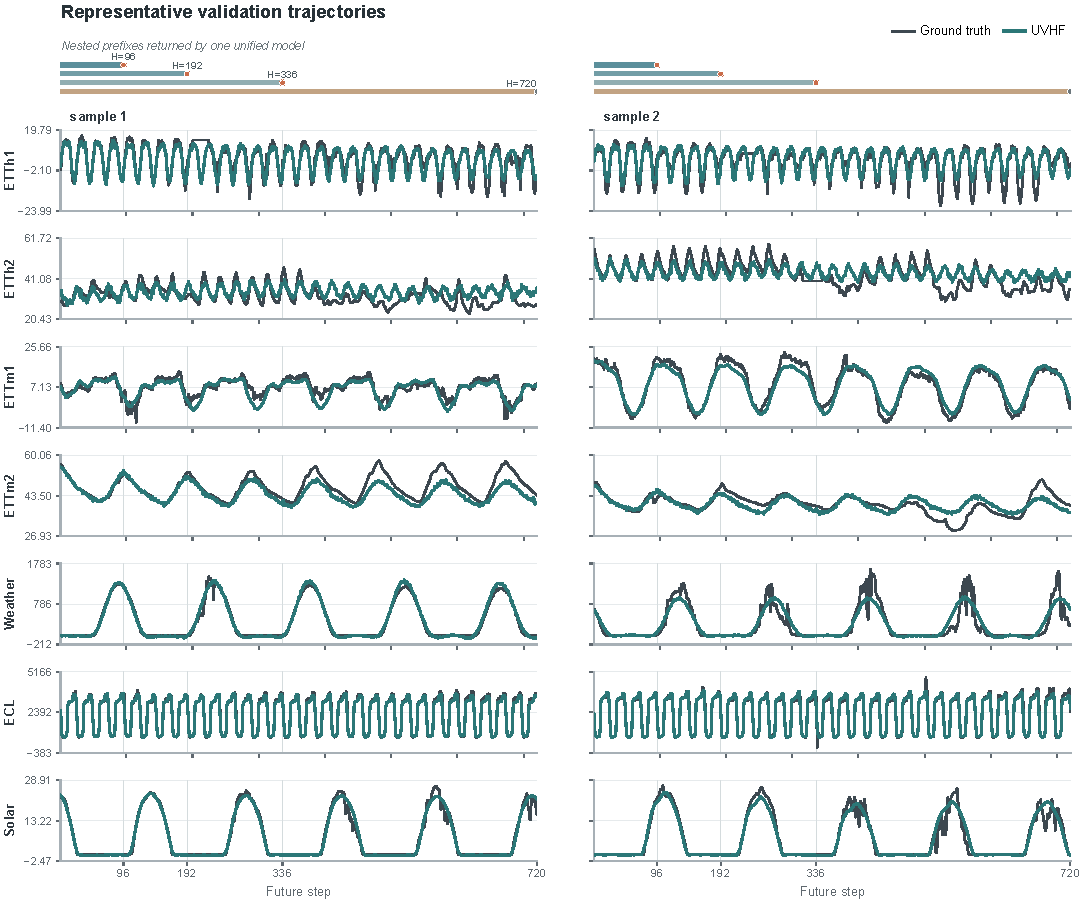
\includegraphics[width=1.00\textwidth]{figure_c1_uvhf_varied_horizon_forecasts.pdf}
\caption{Visualization of varied-horizon forecasts across seven datasets. The dark curve denotes the ground truth and the teal curve denotes the prediction from UVHF. Two validation examples are shown for each dataset. The paired rulers and vertical guides identify the four supported prediction lengths.}
\label{fig:appendix-visualization}
\end{figure}
%% END INLINED UVHF APPENDICES

%% For citations use:
%%       \cite{<label>} ==> [1]

%%
% Example citation, See \cite{lamport94}.

%% If you have bib database file and want bibtex to generate the
%% bibitems, please use
%%
 \bibliographystyle{elsarticle-num}
 \bibliography{ref}

%% else use the following coding to input the bibitems directly in the
%% TeX file.

%% Refer following link for more details about bibliography and citations.
%% https://en.wikibooks.org/wiki/LaTeX/Bibliography_Management

% \begin{thebibliography}{00}

% %% For numbered reference style
% %% \bibitem{label}
% %% Text of bibliographic item

% \bibitem{lamport94}
%   Leslie Lamport,
%   \textit{\LaTeX: a document preparation system},
%   Addison Wesley, Massachusetts,
%   2nd edition,
%   1994.

% \end{thebibliography}
\end{document}

\endinput
%%
%% End of file `elsarticle-template-num.tex'.
